
\chapter{Desenvolvimento}

Este capítulo apresenta a visão geral do jogo proposto, seus requisitos e principais elementos, como personagens e ambientes. Também são detalhados os objetivos e mecânicas do jogo e suas cenas.

\section{Visão Geral}

O jogo é chamado ``Mistério Financeiro: A Jornada de Chico''. No início o protagonista Chico se depara com o mistério das despesas crescentes e do desaparecimento de moedas na papelaria de sua família. Motivado por um senso de responsabilidade, ele decide investigar o caso. A investigação começa pelo porão da loja, um local pouco visitado pela sua família.

A narrativa avança através de uma série de desafios e escolhas que Chico deve enfrentar. Essas decisões vão desde escolhas cotidianas, como a compra de um relógio, até interações complexas com personagens, como seu amigo Vicente. Cada escolha tem um impacto na história e nas lições de economia e gestão financeira apresentadas.

À medida que Chico investiga, ele descobre várias causas para os problemas financeiros da papelaria, desde descuidos simples até ações mal-intencionadas de terceiros. O jogo ressalta a importância da atenção aos detalhes e do controle de gastos para a saúde financeira de um negócio.

O jogo é estruturado de forma interativa, oferecendo múltiplos finais baseados nas decisões do jogador ao longo de sua experiência. Isso enfatiza a relevância de escolhas responsáveis e informadas, tanto no jogo quanto na vida real. Neste sentido, o jogo incorpora um forte elemento educacional, enfatizando conceitos de gestão financeira. Ele ensina sobre a importância do planejamento financeiro, economia e investimentos, incentivando os jogadores a refletirem sobre suas próprias decisões financeiras.

\section{Requisitos de Software}

\subsection*{Requisitos Funcionais}
\begin{itemize}
	\item RF1. O jogo deve oferecer uma interface gráfica interativa, simbolizando os diferentes ambientes da história de Chico.
	\item RF2. Incluir um sistema de diálogo interativo com personagens, como Seu Mário, Vicente, Luiza, entre outros.
	\item RF3. Permitir que o jogador faça escolhas que influenciam o desenvolvimento da história e interações com personagens.
	\item RF4. Permitir a compra e uso de itens para progredir na narrativa, principalmente se tratando da lanterna que será usada para verificar o porão.
	\item RF5. Apresentar múltiplos finais com base nas decisões tomadas pelo jogador, influenciadas pelas interações com personagens.
	\item RF6. Incorporar elementos de educação financeira dentro da narrativa e desafios, utilizando situações da história de Chico como exemplos.
\end{itemize}

\subsection*{Requisitos Não Funcionais}
\begin{itemize}
	\item RNF1. O jogo deve ter uma interface gráfica atrativa e intuitiva, adequada para a faixa etária do 5º ano do Ensino Fundamental.
	\item RNF2. O jogo deve ser otimizado para um desempenho fluido, sem atrasos ou erros técnicos.
	\item RNF3. O jogo deve ser compatível com a plataforma Windows, MacOS e Web.
	\item RNF4. O jogo deve ter uma trilha sonora e efeitos sonoros imersivos, complementando a experiência visual.
\end{itemize}

\subsection*{Regras de Negócio}
\begin{itemize}
	\item RN1. A história deve se adaptar e mudar com base nas escolhas feitas pelo jogador (RF3, RF5).
	\item RN2. Os desafios e enigmas devem ser integrados na história e contribuir para o aprendizado sobre finanças (RF4, RF6).
	\item RN3. Os diálogos e interações com personagens devem oferecer pistas e informações relevantes para a progressão da história (RF2).
	\item RN4. O jogo deve promover a conscientização sobre gestão financeira e economia de forma lúdica e educativa (RF6).
	\item RN5. Os elementos e enredo do jogo devem seguir a história 1 do livro 5 da ENEF, garantindo alinhamento com os princípios educativos estabelecidos.
\end{itemize}

\section{Elementos do Jogo}

\subsection{Personagens e Ambientes}
Esta seção detalha os personagens não jogáveis (NPCs, do inglês \textit{non-player character}) e os ambientes (também chamados de \textit{mapas}) que serão fundamentais para a narrativa e jogabilidade do jogo. Cada NPC e mapa pode ser acompanhado de uma imagem e uma descrição detalhada para melhor imersão e compreensão do jogador.

O jogo apresenta os NPCs apresentados na Figura~\ref{fig:npcs}. Abaixo, é fornecida uma descrição para cada um deles.

\medskip\noindent \textbf{Seu Mário.}\quad Pai de Chico, dedicado dono da papelaria da família. Enfrenta desafios financeiros e tenta manter o negócio próspero.

\medskip\noindent \textbf{Pai do Vicente.}\quad Aparece na história para repreender seu filho por envolvimento em furtos, refletindo preocupação paterna diante da situação indesejada.

\medskip\noindent \textbf{Atendente da Loja de Itens.}\quad Caracterizado como um comerciante prestativo, interage com Chico durante a compra do seu relógio.

\medskip\noindent \textbf{Vicente.}\quad Colega de escola de Chico, conhecido por seu comportamento provocativo e envolvimento em pequenos furtos.

\medskip\noindent \textbf{Luiza.}\quad Melhor amiga de Chico, sempre oferecendo apoio e aconselhamento nas aventuras e desafios enfrentados por ele.

\medskip\noindent \textbf{Maria José.}\quad Mãe de Chico, auxilia na papelaria e compartilha das preocupações financeiras da família.

\medskip\noindent \textbf{Josimar.}\quad Funcionário da papelaria, inicialmente suspeito de furto, revelando-se inocente e um aliado importante.

\medskip\noindent \textbf{Ratazana.}\quad Uma ameaça inesperada no porão da papelaria, adicionando suspense e desafios físicos à narrativa.

\medskip\noindent \textbf{Atendente do Hospital.}\quad Representa um ponto de contato no cenário hospitalar, caso Chico necessite de cuidados médicos devido ao ataque da ratazana.

\medskip\noindent \textbf{Médico.}\quad Figura de cuidado e autoridade, que atende Chico no hospital após eventuais incidentes.

\medskip\noindent \textbf{Atendente da Loja de Ferragens.}\quad Ajuda Chico na aquisição da lanterna, útil durante suas investigações.

\medskip\noindent \textbf{Cida.}\quad Irmã mais nova de Chico, envolvida nos dilemas familiares e curiosa sobre os mistérios da papelaria.

\medskip\noindent \textbf{Personagens não nomeados (4).}\quad Personagens secundários, aparecem apenas para compor algumas cenas, como o encontro com os amigos da escola na lanchonete.


\begin{figure}[ht]
	\centering
	\caption{Imagens de cada NPC.}
	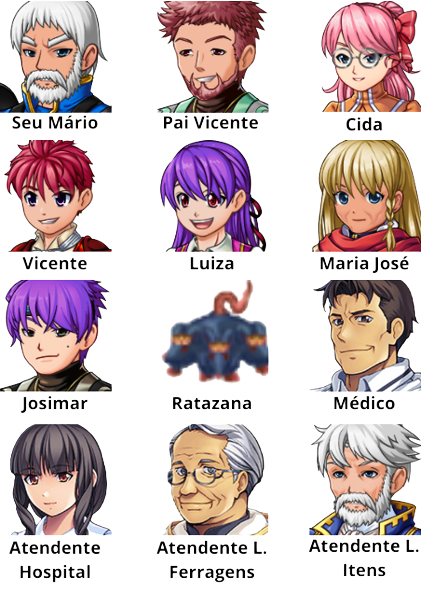
\includegraphics[scale=1.0]{Textuais/Pictures/NPC-Todos.png}
	\fonte{Criado pelo autor.}\label{fig:npcs}
\end{figure}

\newpage

\bigskip\medskip
O jogo ainda apresenta nove ambientes, os quais estão apresentados nas Figuras~\ref{fig:mundo-chico}~--~\ref{fig:hospital}. Os detalhes de cada ambiente são fornecidos abaixo.

\medskip\noindent \textbf{Mundo do Chico.}\quad O cenário geral da aventura, que inclui a vizinhança, ruas e locais frequentados por Chico e seus amigos (Figura~\ref{fig:mundo-chico}).

\medskip\noindent \textbf{Casa do Chico.}\quad Espaço de união e diálogo da família, proporcionando um contraste com as áreas de mistério e aventura (Figura~\ref{fig:casa-chico}).

\medskip\noindent \textbf{Loja de Itens.}\quad Estabelecimento onde Chico adquire itens como o relógio (Figura~\ref{fig:loja-itens}).

\medskip\noindent \textbf{Lanchonete.}\quad Espaço social para Chico e seus amigos, propício para conversas e desenvolvimento de subtramas (Figura~\ref{fig:lanchonete}).

\medskip\noindent \textbf{Loja de Ferragens.}\quad Fornecedora da lanterna para as investigações de Chico (Figura~\ref{fig:loja-ferragens}).

\medskip\noindent \textbf{Papelaria da Família.}\quad Coração da trama, onde muitos dos mistérios e desafios se concentram (Figura~\ref{fig:papelaria-familia}).

\medskip\noindent \textbf{Cozinha da Papelaria.}\quad Local onde Chico encontra o Josimar e faz descobertas, como o problema com a geladeira (Figura~\ref{fig:cozinha-papelaria}).

\medskip\noindent \textbf{Porão da Papelaria.}\quad Ambiente sombrio e cheio de mistérios, onde Chico enfrenta a Ratazana (Figura~\ref{fig:porao-papelaria}).

\medskip\noindent \textbf{Hospital.}\quad Local de cuidado e recuperação, podendo ser cenário de eventos dramáticos, como o ataque da ratazana (Figura~\ref{fig:hospital}).


\begin{figure}[!htbp]
	\centering
	\caption{Mapa Mundo Chico.}
	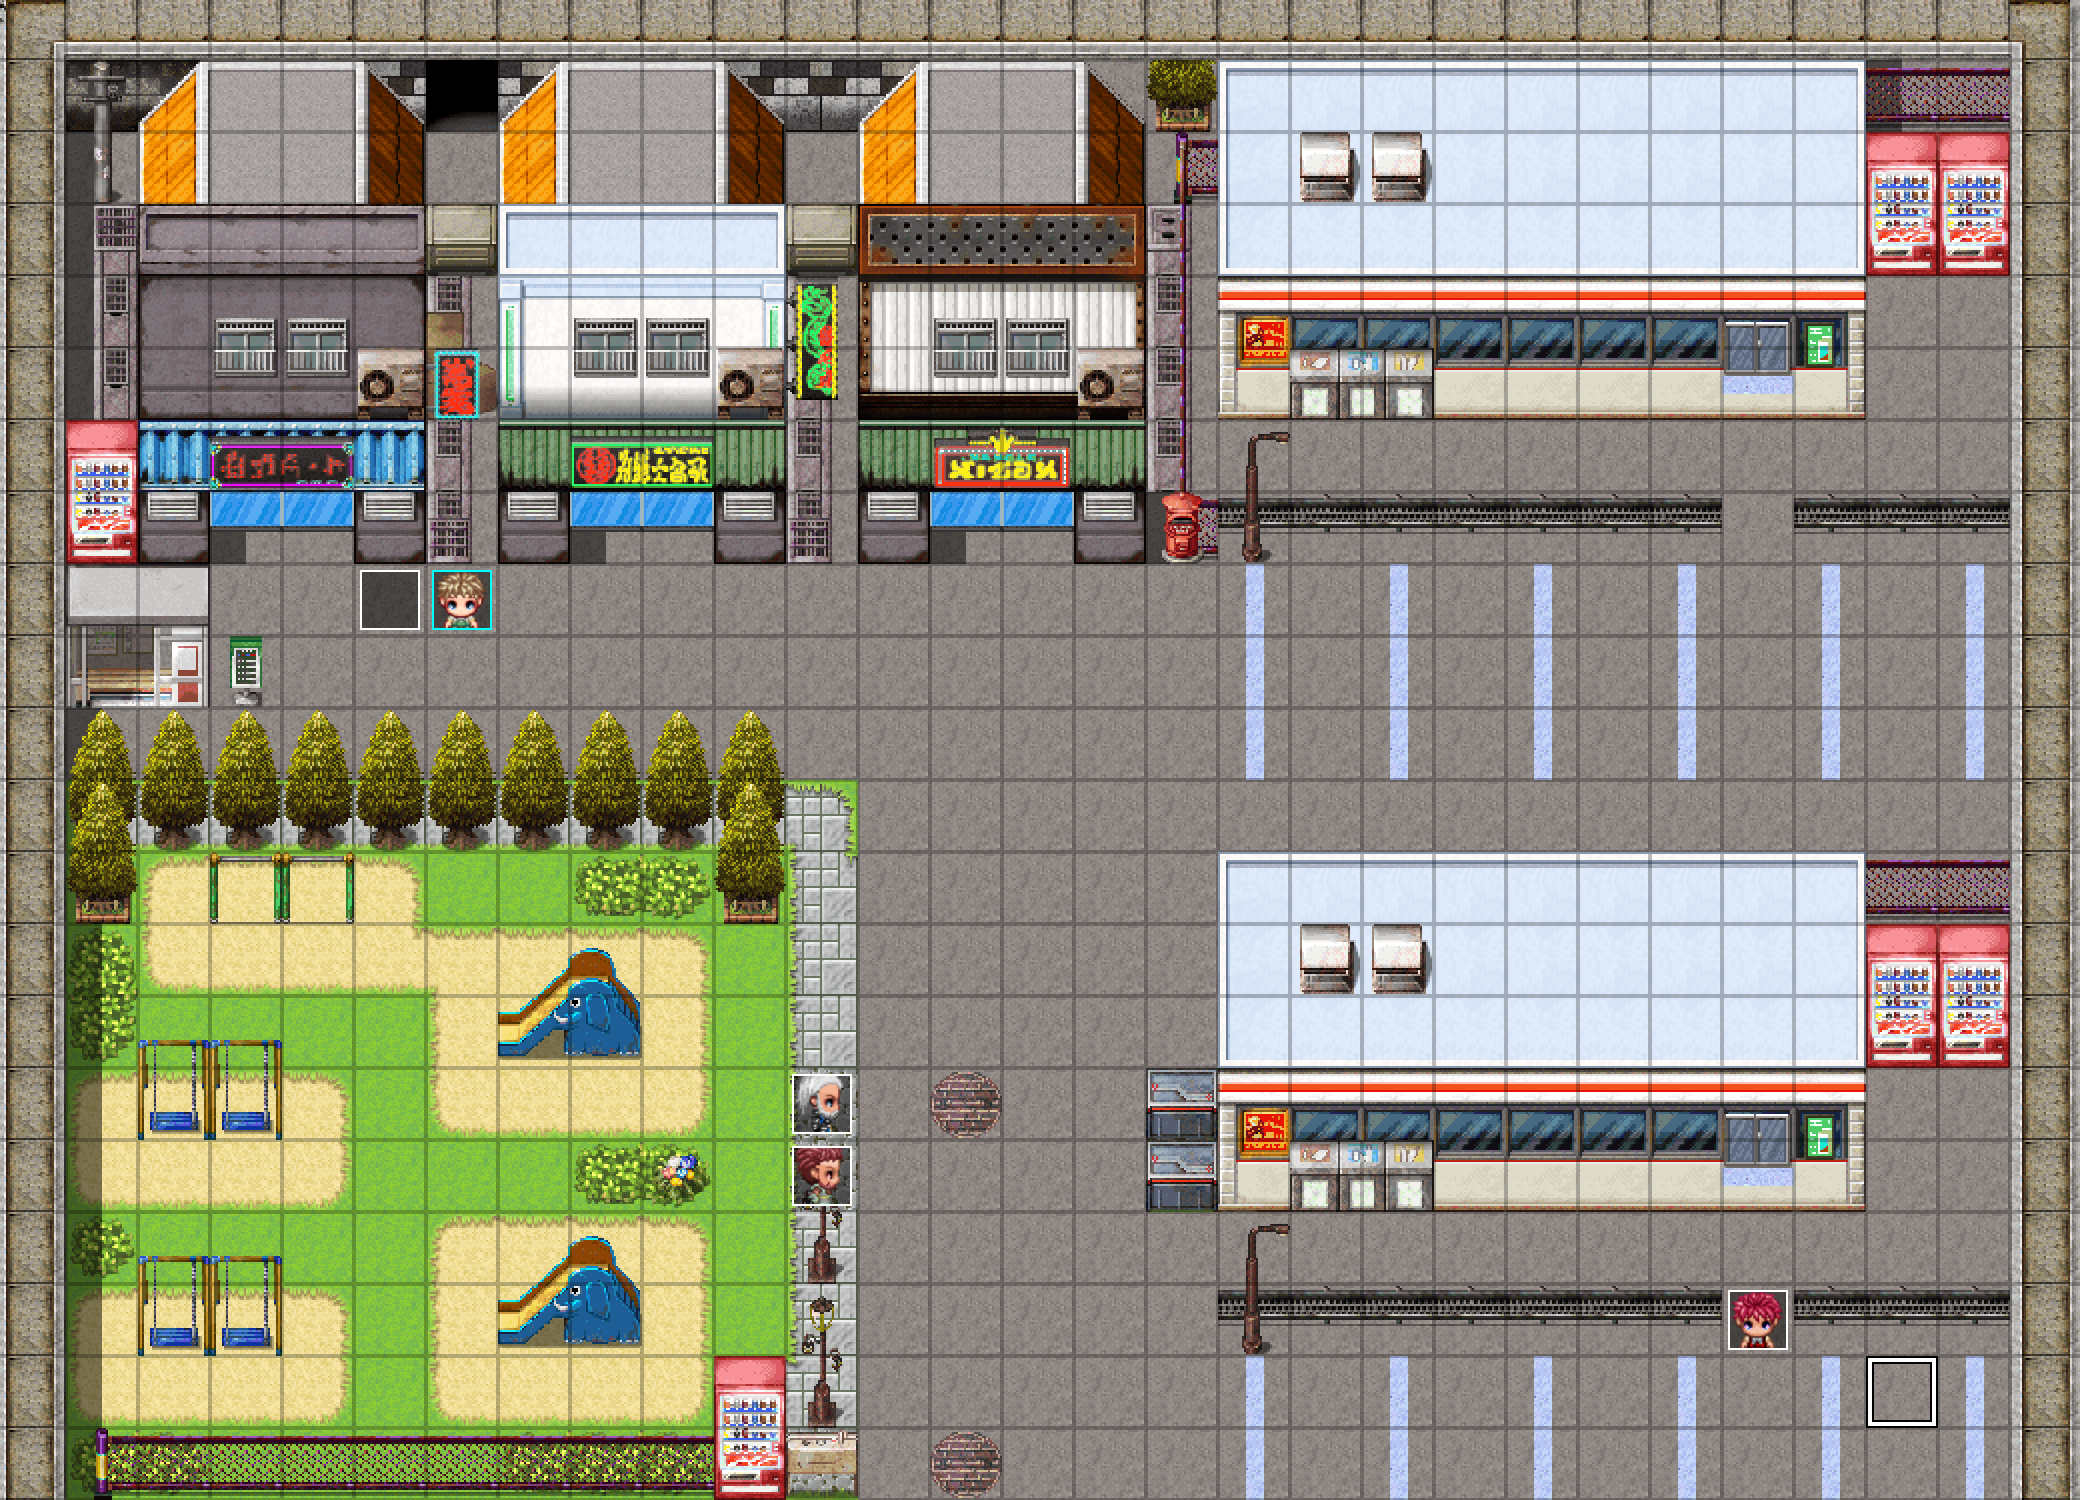
\includegraphics[scale=0.4]{Textuais/Pictures/Mundo_chico.png}
	\fonte{Criado pelo autor com base nos modelos fornecidos pelo RPG Maker MZ.}\label{fig:mundo-chico}
\end{figure}

\begin{figure}[!htbp]
	\centering
	\caption{Mapa da casa do Chico.}
	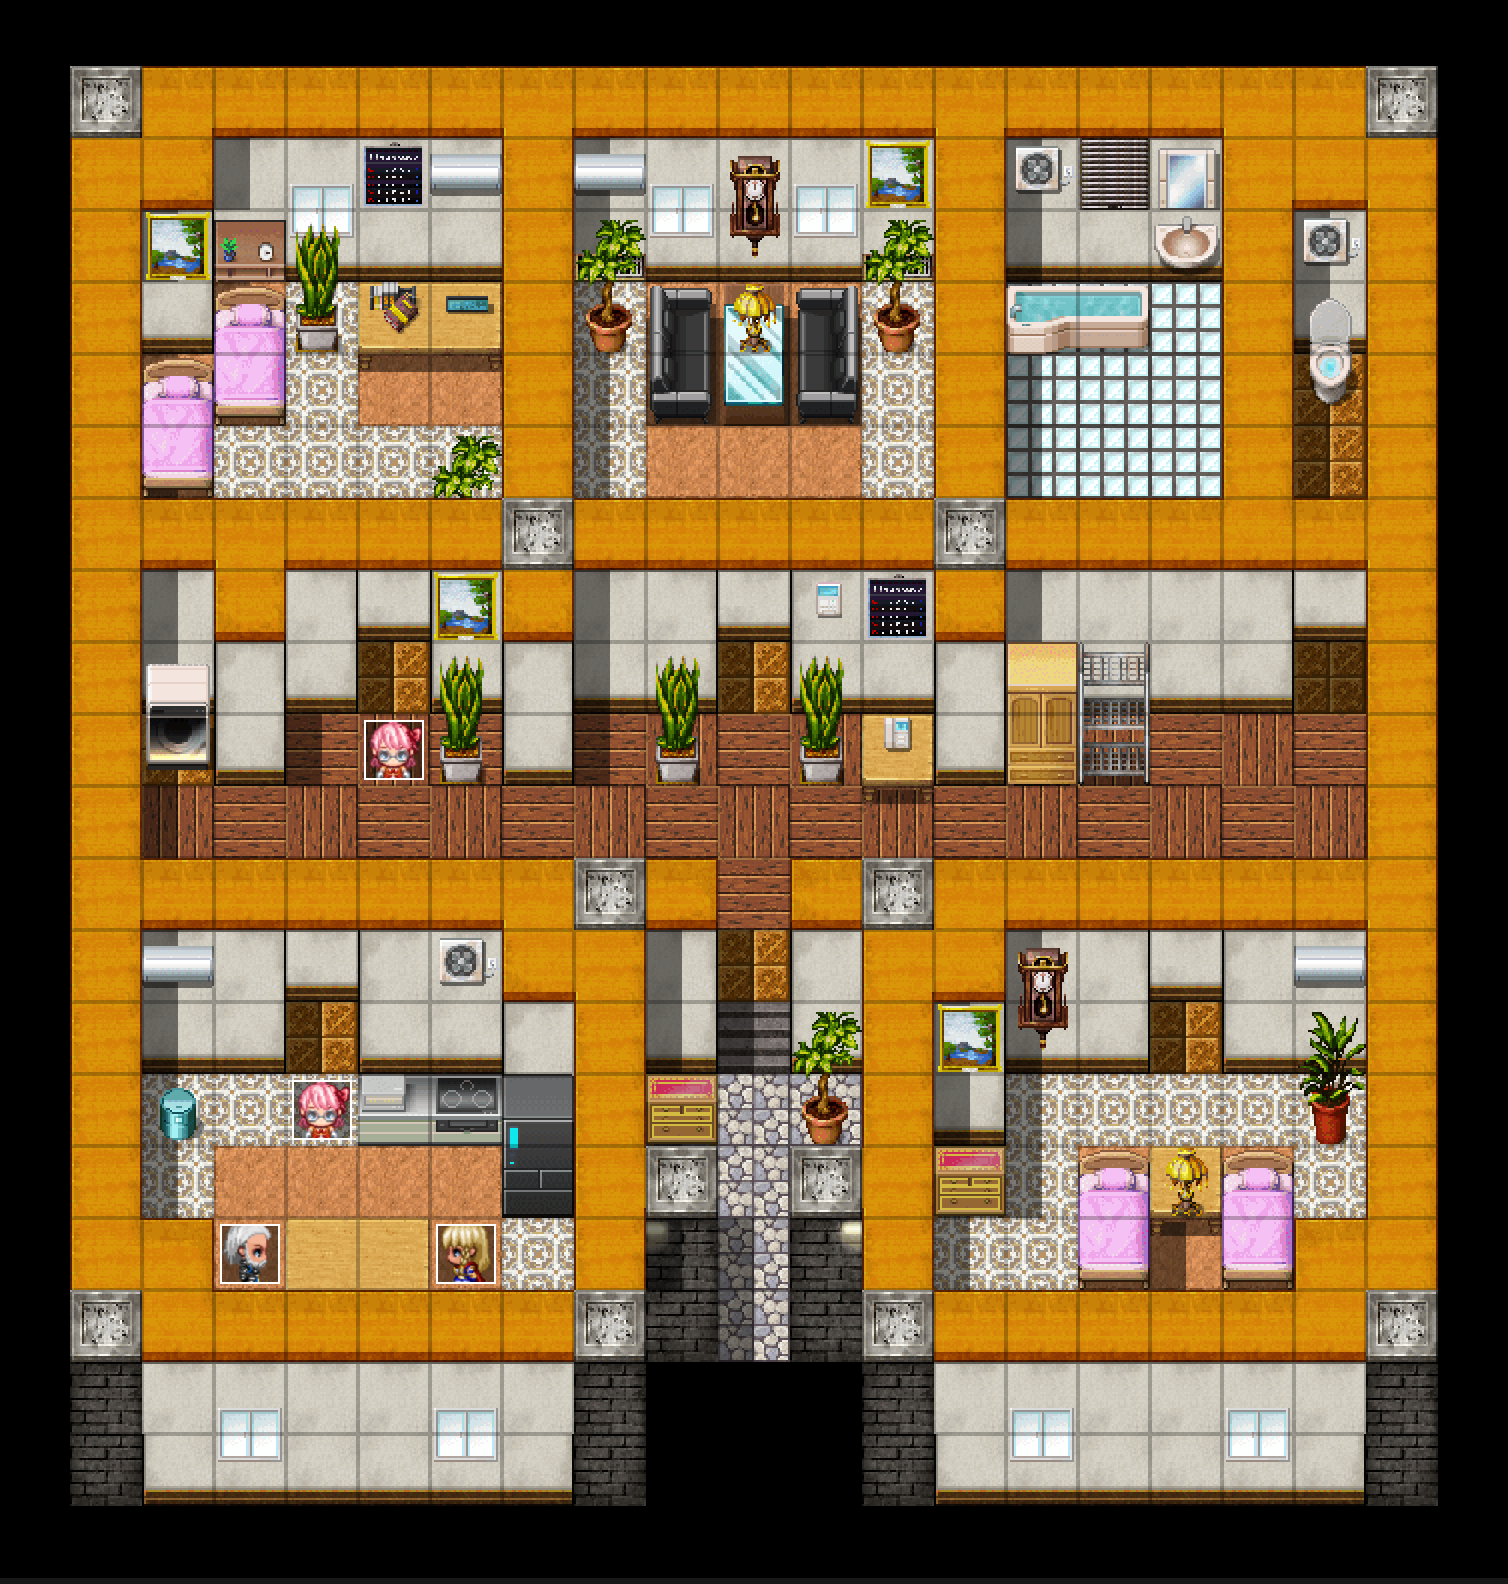
\includegraphics[scale=0.35]{Textuais/Pictures/Casa_chico.png}
	\fonte{Criado pelo autor com base nos modelos fornecidos pelo RPG Maker MZ.}\label{fig:casa-chico}
\end{figure}

\begin{figure}[!htbp]
	\centering
	\caption{Mapa Loja de Itens.}
	\includegraphics[scale=0.5]{Textuais/Pictures/Loja_itens.png}
	\fonte{Criado pelo autor com base nos modelos fornecidos pelo RPG Maker MZ.}\label{fig:loja-itens}
\end{figure}

\begin{figure}[!htbp]
	\centering
	\caption{Mapa Lanchonete.}
	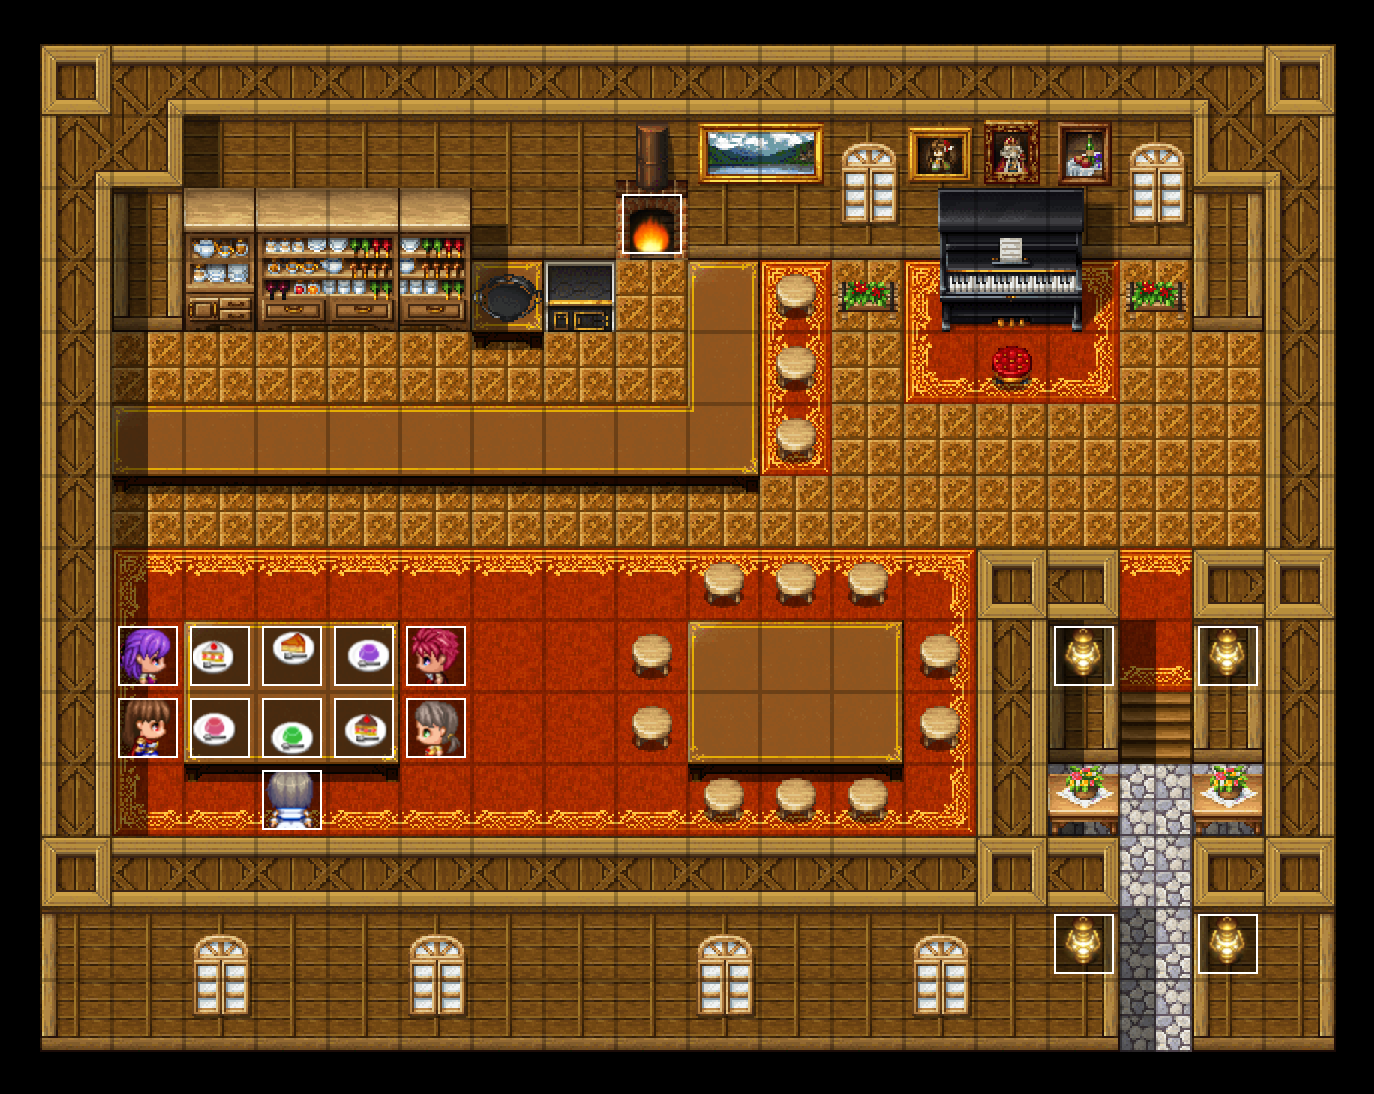
\includegraphics[scale=0.5]{Textuais/Pictures/Lanchonete.png}
	\fonte{Criado pelo autor com base nos modelos fornecidos pelo RPG Maker MZ.}\label{fig:lanchonete}
\end{figure}

\begin{figure}[!htbp]
	\centering
	\caption{Mapa da loja de ferragens.}
	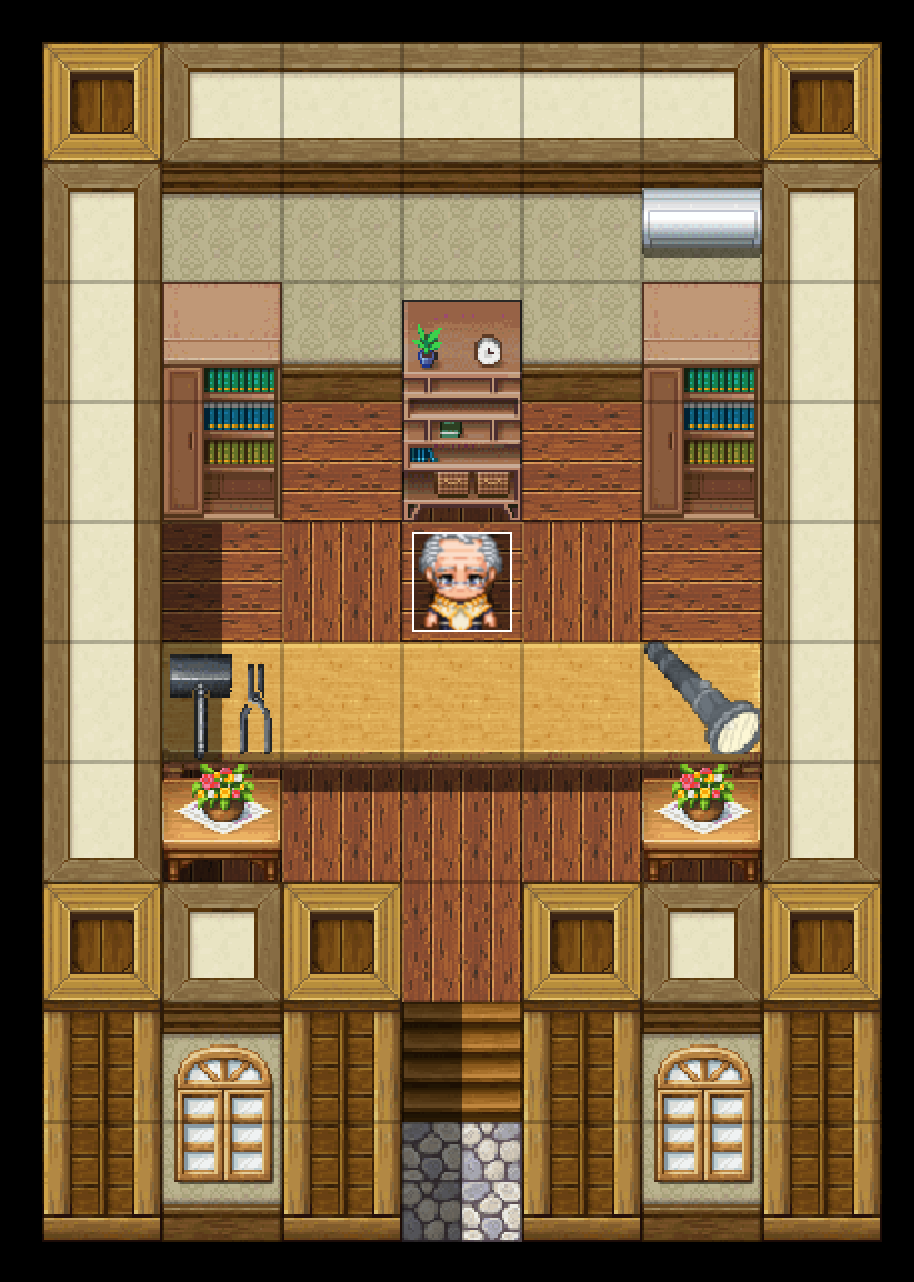
\includegraphics[scale=0.45]{Textuais/Pictures/Loja_Ferragens.png}
	\fonte{Criado pelo autor com base nos modelos fornecidos pelo RPG Maker MZ.}\label{fig:loja-ferragens}
\end{figure}

\begin{figure}[!htbp]
	\centering
	\caption{Mapa Papelaria.}
	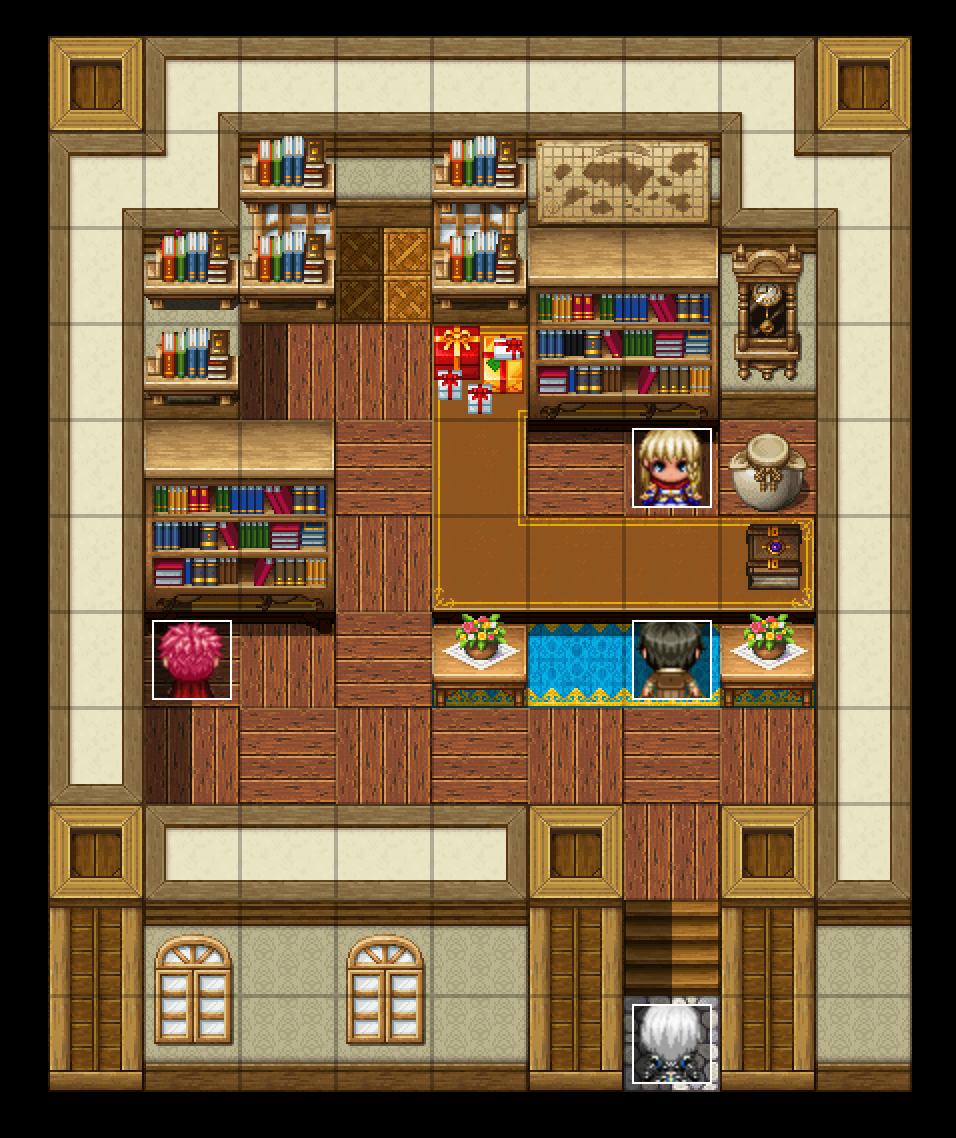
\includegraphics[scale=0.45]{Textuais/Pictures/Papelaria_Familia.png}
	\fonte{Criado pelo autor com base nos modelos fornecidos pelo RPG Maker MZ.}\label{fig:papelaria-familia}
\end{figure}

\begin{figure}[!htbp]
	\centering
	\caption{Mapa da cozinha da papelaria.}
	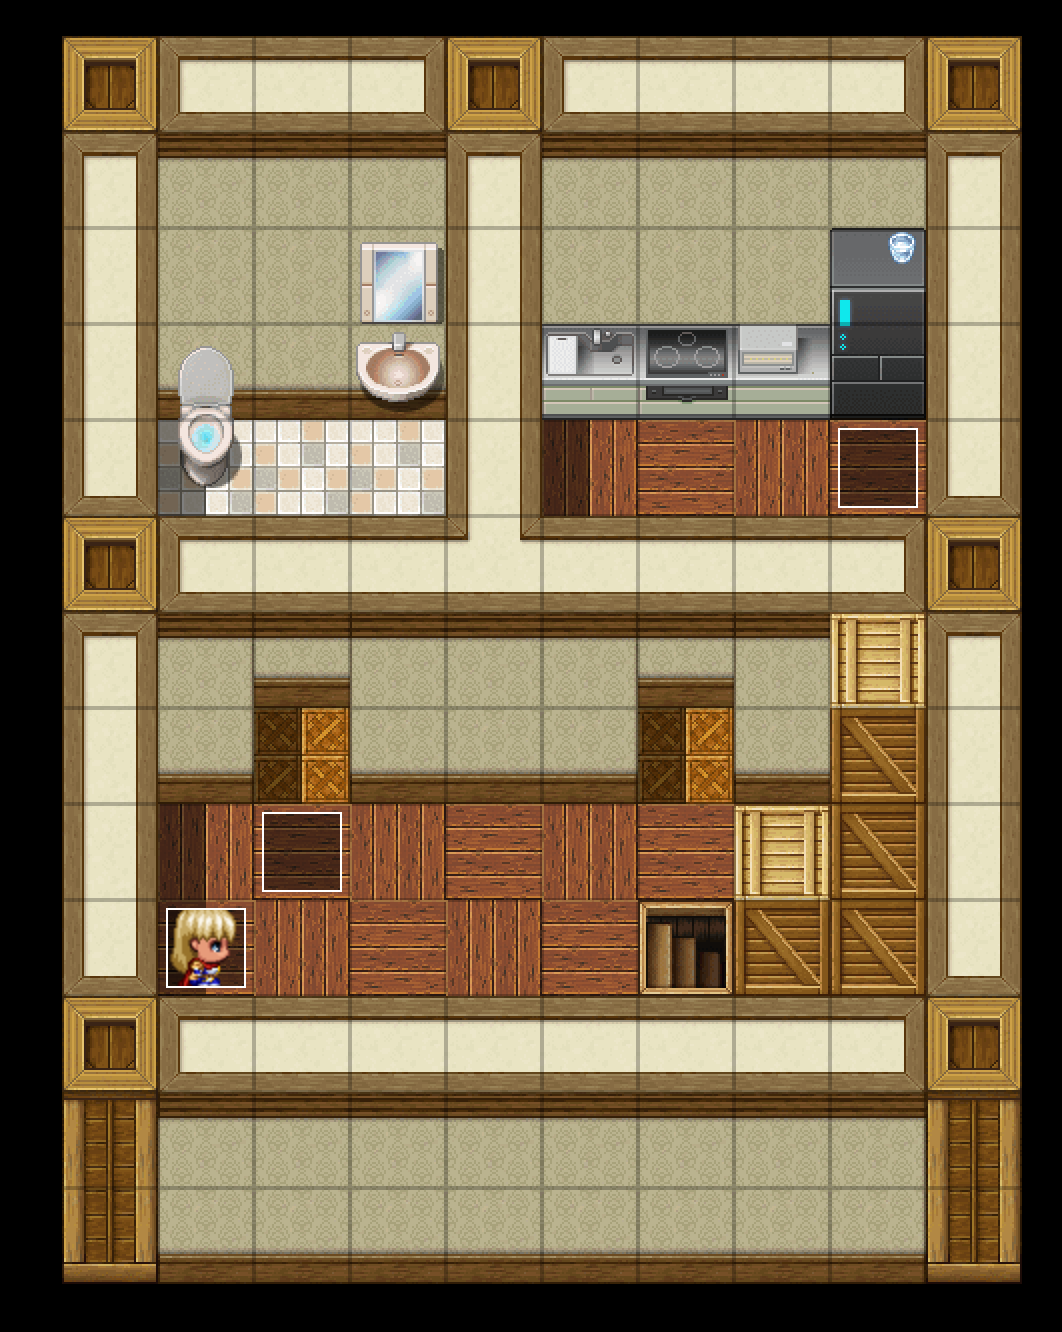
\includegraphics[scale=0.5]{Textuais/Pictures/Cozinha_papelaria.png}
	\fonte{Criado pelo autor com base nos modelos fornecidos pelo RPG Maker MZ.}\label{fig:cozinha-papelaria}
\end{figure}

\begin{figure}[!htbp]
	\centering
	\caption{Mapa do porão da papelaria.}
	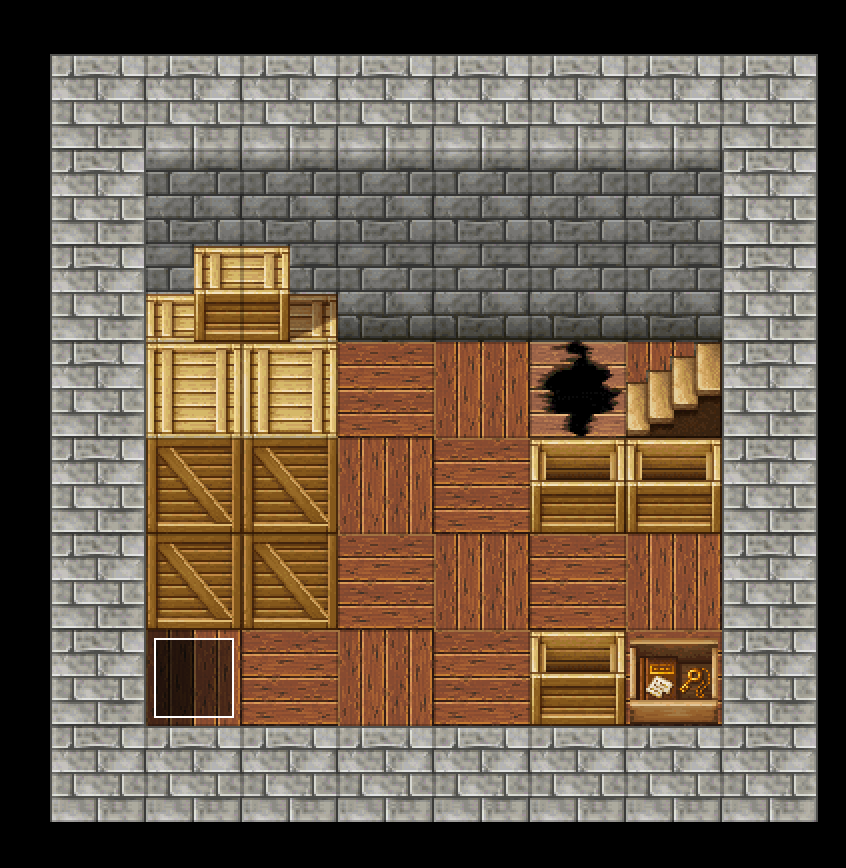
\includegraphics[scale=0.5]{Textuais/Pictures/Porao_papelaria.png}
	\fonte{Criado pelo autor com base nos modelos fornecidos pelo RPG Maker MZ.}\label{fig:porao-papelaria}
\end{figure}

\begin{figure}[!htbp]
	\centering
	\caption{Mapa do hospital.}
	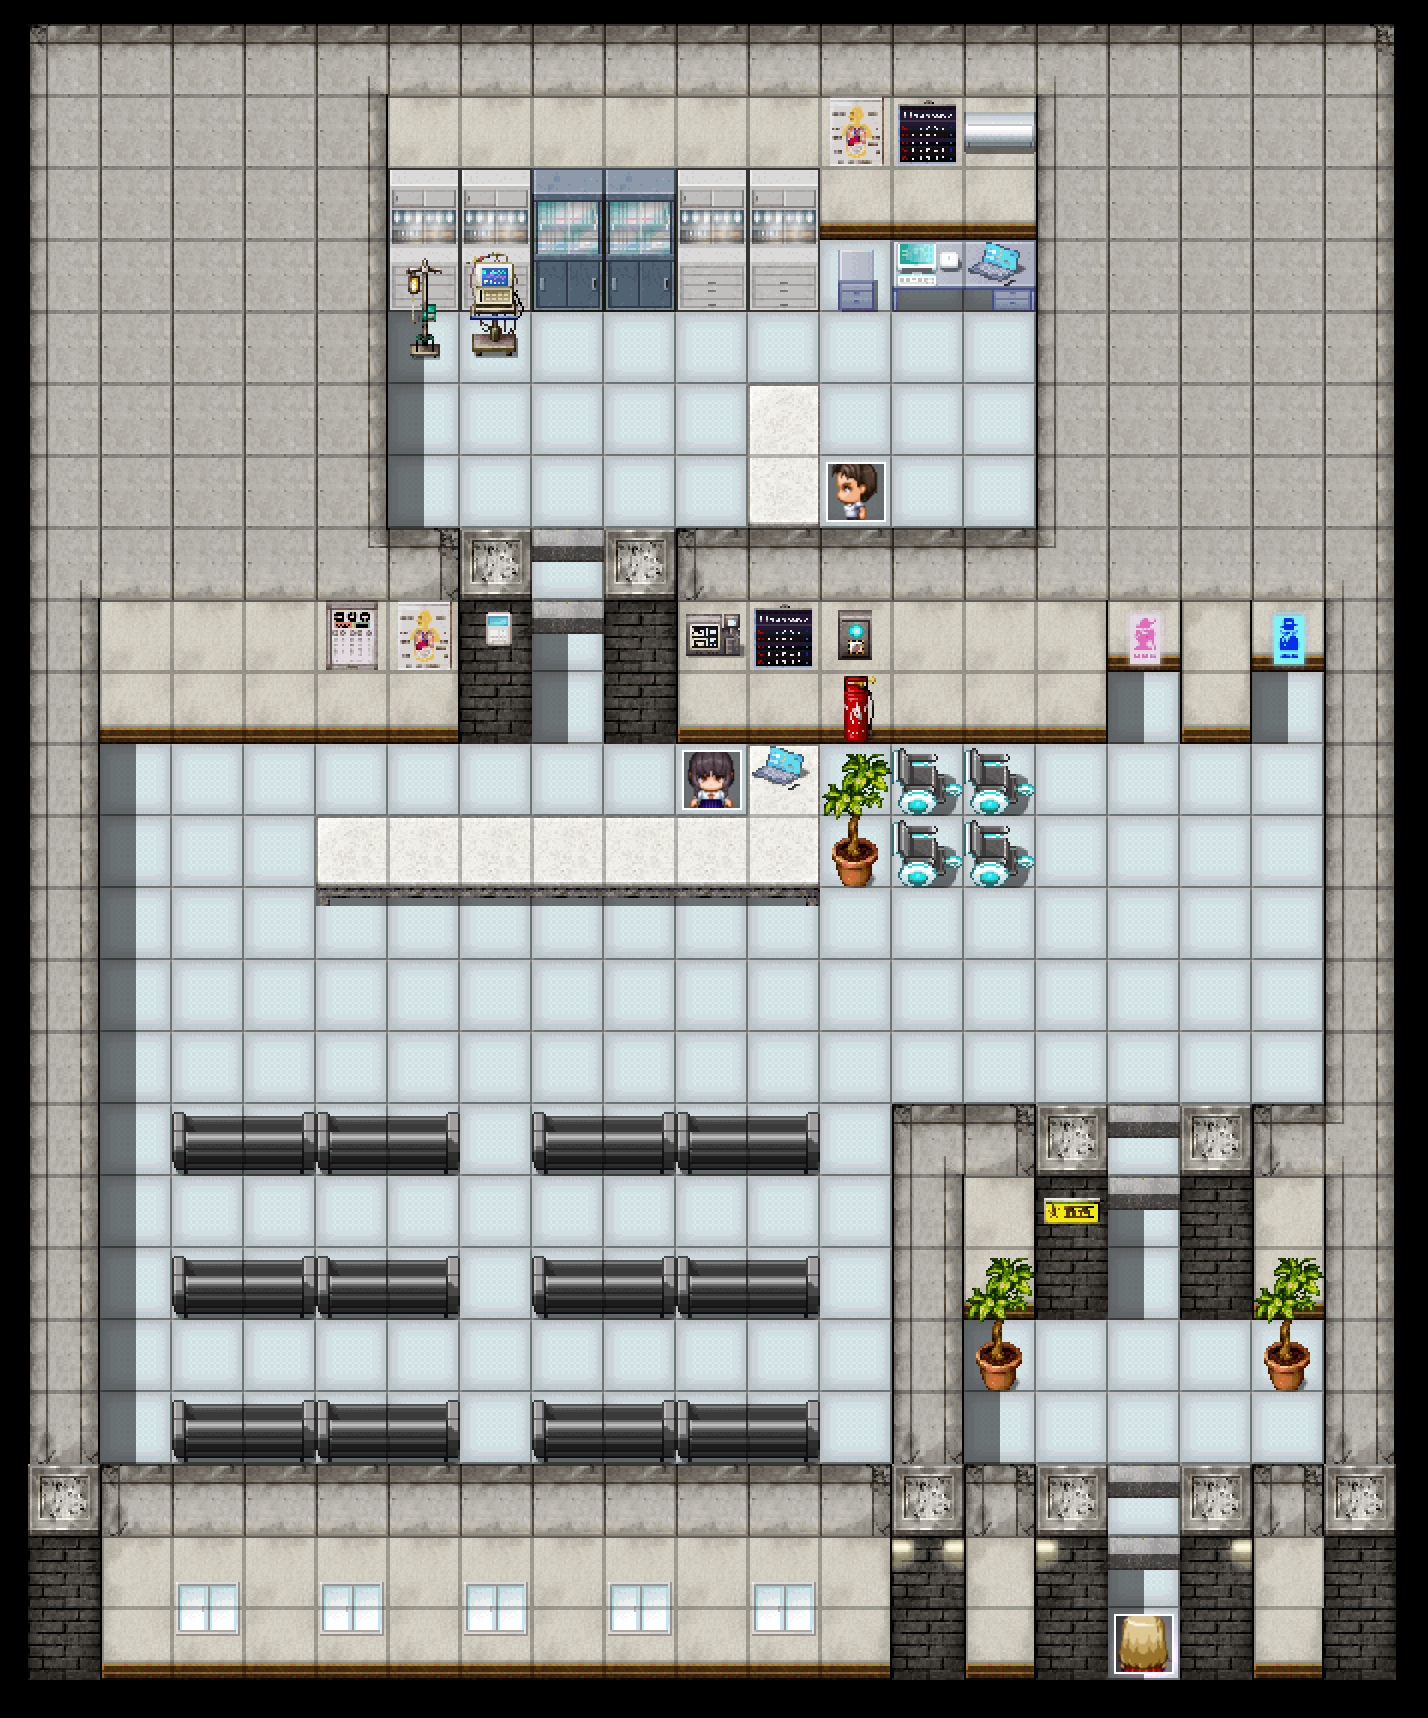
\includegraphics[scale=0.4]{Textuais/Pictures/Hospital.png}
	\fonte{Criado pelo autor com base nos modelos fornecidos pelo RPG Maker MZ.}\label{fig:hospital}
\end{figure}

\newpage

\subsection{Objetivos do Jogo}

No jogo que será desenvolvido no presente trabalho, os jogadores embarcam em uma aventura repleta de desafios e descobertas ao lado do jovem protagonista, Chico. O jogo é estruturado em torno de objetivos claros e progressivos:

\medskip\noindent \textbf{Resolução do Mistério Financeiro.}\quad O objetivo principal é solucionar o mistério do aumento súbito nas despesas da papelaria da família e o desaparecimento de moedas. Chico deve conversar com os personagens e tomar decisões informadas para chegar ao fundo do problema.

\medskip\noindent \textbf{Tomada de Decisões Estratégicas.}\quad Em várias etapas, os jogadores são apresentados a cenários onde devem fazer escolhas que afetarão o rumo da história. Por exemplo, a decisão de qual relógio comprar, como reagir a Vicente ou qual local investigar primeiro.

\medskip\noindent \textbf{Promoção da Educação Financeira.}\quad Através da narrativa, o jogo visa educar os jogadores sobre a importância da gestão financeira, economia e o valor do dinheiro. Os jogadores são incentivados a pensar sobre como pequenas economias podem acumular ao longo do tempo e fazer uma grande diferença.

\medskip\noindent \textbf{Chegar a uma Conclusão Satisfatória.}\quad Dependendo das decisões tomadas, os jogadores podem chegar a diferentes finais. O objetivo é guiar Chico e sua família a uma resolução positiva, onde o mistério é solucionado, a papelaria é salva e as lições aprendidas são aplicadas na vida real.


\subsection{Mecânicas do Jogo}

\medskip\noindent \textbf{Escolhas e Consequências.}\quad O jogo se baseia em uma narrativa interativa, na qual o jogador enfrenta diferentes cenários e situações e deve fazer escolhas que afetarão o rumo da história. Cada escolha pode levar a diferentes resultados, e o jogador deve ponderar as consequências antes de tomar uma decisão.

\medskip\noindent \textbf{Atributos do Personagem.}\quad O personagem principal, Chico, possui atributos como rapidez e agilidade. Estes atributos podem influenciar a capacidade do jogador de superar certos desafios. Por exemplo, se Chico tem uma alta rapidez, ele pode ser capaz de fugir de uma ratazana no porão.

\medskip\noindent \textbf{Pontos de Bônus.}\quad Os jogadores começam com uma quantidade de pontos de bônus que podem ser usados para aumentar os atributos de Chico. Eles devem decidir ao iniciar o jogo como gastar seus 3 pontos bônus.

\medskip\noindent \textbf{Narrativa Não Linear.}\quad Dependendo das escolhas feitas, os jogadores podem experimentar diferentes cenários e resultados.

\medskip\noindent \textbf{Educação Financeira.}\quad Embora o jogo seja uma aventura, há um subtexto educacional sobre gestão financeira. O jogo destaca a importância de economizar, gerenciar despesas e considerar o valor do dinheiro.

\medskip\noindent \textbf{Desafios e Obstáculos.}\quad Os jogadores enfrentarão desafios variados, desde decisões financeiras (como a escolha do relógio) até obstáculos físicos (como a ratazana no porão).

\medskip\noindent \textbf{Interações Sociais.}\quad Chico interage com vários personagens, e essas interações podem fornecer pistas, criar conflitos ou ajudar na resolução do mistério.

\medskip\noindent \textbf{Conclusão Variável.}\quad O jogo tem múltiplos finais possíveis, dependendo das decisões tomadas pelo jogador ao longo da história.

Em resumo, é um jogo de aventura narrativa com elementos educacionais e de tomada de decisão, onde as escolhas do jogador afetam diretamente o desfecho da história. É uma mistura envolvente de exploração, interatividade e aprendizado.

\subsection{Cenas}

\subsubsection{\textit{\textbf{Cena 1}}}

A sua família conseguiu tudo que tem com muito trabalho e perseverança, e evitando gastar demais. Assim, montaram uma papelaria e compraram um apartamento perto dela, o que permite que, seu pai, Seu Mário possa ir até o trabalho a pé. Sua mãe, Maria José, reveza com seu pai o trabalho na papelaria; Você e sua irmã Maria Aparecida (Cida) gostam de ajudar, mas como seus pais querem que vocês deem preferência aos estudos, eles contrataram um funcionário, o Josimar.

Quando você chega da escola, encontra o seu pai e a sua mãe conversando muito preocupados:

-- Não sei mais o que fazer, Maria. As contas não param de subir e já procurei as moedas por toda parte e não encontro!
-- Você não está achando que o Josimar...
-- De forma alguma, eu confio no rapaz. Mas, não sei o que fazer. Vamos ter que apertar o cinto, cortar despesas até a situação melhorar. Estamos chegando perto do Dia da Criança, então as vendas devem aumentar.
-- Posso ajudar, pai? -- você pergunta ansioso.
-- Pode indo fazer seu dever de casa e se concentrando nos estudos. Deixa esses problemas de adulto com a gente.

Você vai chateado para o quarto, afinal já tem 11 anos e não é mais uma criançinha. Será que seus pais não veem isso, Além do mais, o problema da papelaria também é seu, afinal é dua família! e apesar deles confiarem no Josimar, você toma uma decisão,

-- Vou fazer minhas próprias investigações! Tenho certeza de que deve haver algo no porão, o papai não vai lá desde que a luz queimou no mês passado. As moedas podem estar escondidas lá! Vou comprar uma lanterna e dar uma olhada.

Depois de terminar os deveres de casa, você sai para dar uma volta antes de ir para a papelaria. Sua mãe lhe deu R\$ 50,00 para comprar um relógio novo e você decide fazer isso antes de começar as investigações.

Em poucos minutos você vai de casa até a loja e observa os relógios até que encontra um que parece muito legal: preto, com detalhes em aço, cronômetro, alarme e resistente à água. E custa só R\$ 30,00.

Distraído, não percebe que o Vicente está lá. Um garoto chato da sua escola que vive provocando os outros. Ele está fascinado olhando para um relógio do Major Trovão, que é todo colorido. Você nem gosta muito do desenho do Major Trovão, mas o Vicente e a maior parte da turma adoram. O Vicente te vê e logo provoca:

-- O que veio fazer aqui, Chico? Comprar uma pilha nova para aquele seu relógio velho? Acho melhor você ir no brechó e ver se dá para trocar aquela porcaria por balas!
-- e cai na risada.

Você fica bravo; seria bom dar uma lição nesse chato. O relógio do Major Trovão custa R\$ 45,00 e dessa vez você tem o dinheiro! Se bem que você nem acha o relógio bonito, mas talvez valha a pena comprá-lo só para ver a cara do Vicente e mostrá-lo para o resto da turma.

\subsubsubsection*{Decisões}
\begin{itemize}
	\item \textbf{Se decidir comprar o relógio do Major Trovão, vá para 9.}
	\item \textbf{Se decidir comprar o relógio que você gostou, vá para 4.}
\end{itemize}

\bigskip\medskip

\subsubsection{\textit{\textbf{Cena 2}}}
Você abre a porta com cuidado e desce até o porão, a escada range um pouco. Está muito escuro, mas com a lanterna acesa você consegue ver várias caixas empilhadas umas sobre as outras e sente um leve cheiro de mofo no porão. O pior é um ralo aberto bem no meio do caminho.

-- É melhor avisar meus pais sobre isso. Se der mofo, vamos ter um prejuízo grande com esses cadernos, formulários e livros que não vamos poder vender. E se entrar um bicho por esse ralo? As baratas vão fazer a festa devorando os livros!

Você vai até as caixas e as examina devagar. Na primeira tem uma porção de livros escolares, na segunda, cadernos, na terceira há lápis e borrachas, na quarta encontra formulários. É quando você repara em uma caixa aberta no chão. Curioso, vai até lá dar uma olhada e encontra alguns cadernos, canetas e uma caixinha cheia de moedas.

-- O que será isso? Está parecendo o troco do dia que alguém trouxe aqui para baixo junto com a caixa. Isso deve ser coisa do Josimar.

Nesse momento, um barulho às suas costas lhe dá um calafrio na espinha. Sem perder tempo, você se vira, mira a lanterna na direção do ruído e se depara com uma ratazana em seu ninho com alguns filhotes. Ela avança na sua direção com os dentes arreganhados, pronta para lhe dar uma bela mordida.

Pernas pra que te quero!? Você sai correndo em direção à porta o mais rápido que pode. Se aquela ratazana te alcançar, você pode perder um dedo com a mordida e ainda por cima terá que tomar um monte de injeção para se proteger das doenças que esse bicho deve ter nos dentes.

A ratazana corre no seu encalço, vindo cada vez mais rápida!

\subsubsubsection*{Decisões}
\begin{itemize}
	\item \textbf{Se a sua rapidez for 4 ou mais, vá para 12.}
	\item \textbf{Se a sua agilidade for 3, vá para 5.}
\end{itemize}

\bigskip\medskip

\subsubsection{\textit{\textbf{Cena 3}}}
Você entra na cozinha e encontra o Josimar comendo um sanduíche. A cozinha não é grande, tem uma pequena geladeira, um filtro, uma pia, um armário, uma mesa e três cadeiras. Num canto há várias caixas com as coisas que são usadas com mais frequência. Assim, não se tem que descer a toda hora até o depósito no porão para repor algum item na loja.

Você toma um copo de água, enquanto o Josimar termina o lanche e sai. Já que está ali, você decide examinar as caixas que lá estão, em busca das moedas perdidas, mas nada encontra.

-- Será que é o Josimar quem está sumindo com as moedas? -- você se pergunta.

Quando se vira para guardar o copo, nota que a porta da geladeira está aberta.

-- Estranho... eu tenho certeza de que a fechei depois que peguei a água...

Você vai até lá, fecha a porta da geladeira, depois lava o copo e o guarda no armário. É quando vê alguma coisa reluzindo na prateleira de cima do armário. Depois de pegar a cadeira, você sobe nela e encontra um copo cheio de moedas.

-- Achei! Quem deixou essas moedas aqui? Só pode ter sido o Josimar, para pegá-las depois!

Você se vira pronto para contar a descoberta para sua mãe e toma um grande susto quando vê a porta da geladeira aberta novamente. O que estará acontecendo?

Sua primeira vontade é sair dali correndo, mas você consegue se controlar:

-- O que é isso, Chico? Tenha coragem! Vai lá na geladeira descobrir o que está acontecendo, rapaz!

Você caminha devagar até a geladeira e abre devagarzinho a porta. Depois, com muito cuidado, espia lá dentro.

A geladeira é daquelas que têm um freezer sem porta, o qual está coberto com uma crosta grossa de gelo. A borracha da porta também está meio solta e por isso ela não fecha direito. Você testa abrindo e fechando algumas vezes, e a porta acaba ficando sempre entreaberta.

-- Ora, mas assim essa geladeira está gelando é nada! Está só gastando energia!

Você para e pensa: “Será que a luz da cozinha ficou ligada o dia inteiro? Mas, com essa janela enorme, só precisa de luz elétrica de noite.” Você, então, percebe o quanto de energia elétrica a sua família está desperdiçando só na cozinha.

-- Por isso que a conta de luz subiu tanto. Mas, e as moedas? Ainda falta achar outro tanto!

\subsubsubsection*{Decisões}
\begin{itemize}
	\item \textbf{Se ainda quiser ver o banheiro, vá para 7.}
	\item \textbf{Se ainda não tiver verificado o porão, vá para 6 se não tiver lanterna e para 2 se a tiver.}
\end{itemize}

\bigskip\medskip

\subsubsection{\textit{\textbf{Cena 4}}}
Você decide que o melhor é deixar o Vicente para lá e comprar o relógio do qual gostou. Afinal, o relógio é para você e não para ele. Você compra o relógio pagando R\$ 30,00 e tomando o cuidado de pedir e guardar a nota fiscal. Quando sai da loja, o Vicente não está mais lá.

Você caminha até a papelaria e no caminho encontra com a turma que está indo para a lanchonete comer alguma coisa. Você os acompanha e mostra seu relógio novo, que faz sucesso com o pessoal, o que te deixa bem feliz.

-- Nossa, que relógio lindo! -- exclama Luísa, sua melhor amiga.

-- E nem foi tão caro!

-- Claro que não. O mais legal era o do Major Trovão, mas esse era caro demais para o Chico -- ri Vicente.

-- E quem se importa com o Major Trovão? -- responde Luísa lhe defendendo --
Eu, hein? Virou criancinha, Vicente?

A turma cai na risada, e Vicente sai dali sem graça. Seus pais lhe ensinaram que a gente deve tentar sempre entender e perdoar os outros, mas você não consegue evitar um sorriso que vai de ponta a ponta.

Depois de comer um salgado e um refresco, gastando R\$ 5,00 com o lanche, você se despede da turma e vai até a loja de equipamentos para comprar uma lanterna. Procurando um pouco, você encontra uma muito boa por apenas R\$10,00, e vai direto para a papelaria antes que ela feche.

Você chega com o sol se pondo e entra rápido; passa por sua mãe, que está atendendo a um cliente, e vai direto para os fundos da loja. Nos fundos, tem um banheiro, uma pequena cozinha para as refeições com um mini depósito e a escada para o porão. Você ouve um barulho na cozinha. “O que será isso?

\subsubsubsection*{Decisões}
\begin{itemize}
	\item \textbf{Se decidir investigar o barulho na cozinha, vá para 3.}
	\item \textbf{Se decidir ir direto para o porão, vá para 2.}
\end{itemize}

\bigskip\medskip

\subsubsection{\textit{\textbf{Cena 5}}}
Você sai pela porta e sobe pela escada correndo e gritando o mais que pode. A ratazana lhe segue furiosa escada acima. Ela dá um salto, mas você consegue escapar e grita:

-- Mãe, socorro! É uma ratazana!

Sua mãe aparece no alto da escada brandindo uma vassoura e parte para cima da ratazana. Num primeiro momento, o animal resolve encarar, mas toma uma bela vassourada da sua mãe. A ratazana mostra os dentes, mas sua mãe ergue a vassoura e avança para acabar com ela, que, então, acha por bem cair fora dali e foge correndo de volta para o porão.

Você pega um esfregão e desce pronto para ajudar sua mãe. Mas, ela faz sinal para você voltar e pergunta:

-- O que houve? De onde veio esse bicho?

-- Tem um ralo aberto, e ela deve ter entrado por ele. Tem também um ninho com filhotes.

-- Amanhã, com a luz do dia, vou pedir para o Josimar ir lá tampar o ralo e tirar esse bicho daqui. Mas, o que você foi fazer no porão?

-- Eu estava procurando as moedas que sumiram, achei que podiam estar lá.

-- Que bobagem, menino.

-- Pelo menos eu descobri que o porão está com cheiro de mofo. É melhor ver isso, senão, vamos perder muitos cadernos e livros. E com o ralo aberto, os ratos e as baratas vão fazer a festa com os livros e os cadernos.

-- Bom, nisso você tem razão. Por esse lado, valeu a pena você ter ido ao porão. Vou falar com seu pai. Agora vai tomar um copo de água pra se refazer do susto.

Você sobe a escada e chega até o corredor que dá para a cozinha e o banheiro.

\subsubsubsection*{Decisões}
\begin{itemize}
	\item \textbf{Se ainda não tiver ido para a cozinha, vá para 3.}
	\item \textbf{Se já tiver ido para a cozinha, vá para 7.}
\end{itemize}

\bigskip\medskip

\subsubsection{\textit{\textbf{Cena 6}}}

Você desce até o porão, está bem escuro, afinal o sol já está se pondo, mas essa não é a hora de ter medo. As moedas devem estar lá.

A escada range um pouco, e você abre a porta com cuidado. Consegue ver na escuridão várias caixas empilhadas umas sobre as outras e sente um leve cheiro de mofo no porão.

-- É melhor avisar meus pais sobre isso. Se der mofo, vamos ter um prejuízo grande com esses cadernos, formulários e livros que não vamos poder vender.

Você anda devagar e de repente sente seu pé afundar em algo, tropeça e quase cai de cara no chão. Por sorte não se machuca. O que será esse buraco? Examinando com as mãos, descobre ser um ralo que alguém deixou aberto.

Levantando-se, você vai até as caixas e as examina devagar. Abre uma, olha na outra, move uma terceira de lugar. De repente, sente um calafrio. Olha para cima e vê dois olhos pequenos e vermelhos mirando você. Um ruído estranho sai deles e algo avança na sua direção.

\subsubsubsection*{Decisões}
\begin{itemize}
	\item \textbf{Se a sua agilidade for 3 ou mais, vá para 10.}
	\item \textbf{Se a sua agilidade for 2, vá para 8.}
\end{itemize}

\bigskip\medskip

\subsubsection{\textit{\textbf{Cena 7}}}

Você vai até o banheiro e se depara com o Josimar saindo e contando algumas moedas. Ele sorri para você e vai para a frente da loja para atender o público.

-- Será que é ele? Contando as moedas que conseguiu furtar? -- é o que passa pela sua cabeça.

No banheiro você se depara com várias toalhas de papel no lixo e a torneira aberta, escorrendo água. Você lava as mãos, as seca com apenas duas folhas de papel e nota que a torneira não está fechando direito, por isso ela fica pingando. Aí percebe o quanto você e sua família estão desperdiçando papel e água.

Desperdícios: são gastos que fazemos sem pensar e que pouco ou nada acrescentam à nossa qualidade de vida. Gastar mais do que precisamos, por exemplo, com luz e água, compromete o meio ambiente e faz com que as contas de luz e água sejam maiores do que precisariam ser. O mesmo vale para outros gastos, como comprar coisas que não precisamos, apenas para acompanhar os outros, para impressionar pessoas, por impulso etc. Além disso, gastar muito com coisas que pouco queremos e das quais não precisamos é mais do que perder dinheiro: também é um desperdício ambiental. Tudo o que compramos foi construído com materiais extraídos da natureza, pode ter passado por processos industriais que danificam o meio ambiente e provavelmente foi transportado em algum momento, o que também tem seus impactos ambientais. Além do mais, quando descartado, vira lixo.

Ao sair do banheiro pronto para falar com seu pai sobre como o Josimar gasta papel
para enxugar as mãos e as suas suspeitas de que é ele quem está roubando as moedas
que sumiram, você nota Vicente andando como quem não quer nada pela papelaria.
Da porta do corredor, você consegue vê-lo sem que ele te veja; então decide ficar observando.

Josimar está atendendo a dois clientes ao mesmo tempo, pois sua mãe não se encontra. Vicente pega uma mercadoria, olha o preço, pega outra e fica discretamente observando Josimar. Quando tem certeza de que o empregado não está vendo, Vicente pega várias canetas e mete no bolso. Logo depois, Josimar deixa o troco de um cliente no balcão, que está desatento falando ao celular. Quando Josimar se vira para finalizar o atendimento ao segundo cliente, Vicente vai lá e mete a mão no troco sem que ninguém perceba. Ninguém, exceto você.

Furioso, você grita:

-- Pode parar aí, Vicente!

Todos param surpresos, e Vicente sai correndo. Sem perder tempo, você vai atrás dele.

\subsubsubsection*{Decisões}
\begin{itemize}
	\item \textbf{Se a sua rapidez for 4 ou mais, vá para 11.}
	\item \textbf{Se a sua rapidez for 3 ou menos, vá para 8.}
\end{itemize}

\bigskip\medskip

\subsubsection{\textit{\textbf{Cena 8}}}
Você salta e corre para a porta, então ouve a coisa correndo na sua direção. Você corre o mais que pode, porém está muito escuro. Cadê a porta?! Você se atrapalha todo, tropeça e bate de cara na soleira da porta. Tonto, cai para trás, batendo com as costas no chão.
Quando tenta se erguer, sente uma dor enorme na mão esquerda e sai gritando.

Já na escada, sua mãe aparece, dá um grito e aponta para a sua mão. Você olha e vê horrorizado uma ratazana com os dentes ferrados nela. A ratazana abre a boca, mas sua mãe a acerta com o chinelo, ela cai e volta correndo para o porão.

Sua mão está sangrando muito e a dor é enorme. Sua mãe o leva até o hospital, onde você é atendido e toma uma série de injeções para se proteger das doenças que a ratazana pode ter lhe passado com a mordida. Raiva, por exemplo.

O médico também manda você passar dois dias em observação em casa e repousar bastante. Só lhe resta descansar até ficar bom.

Infelizmente, sua aventura termina aqui, talvez sua irmã tenha melhor sorte em ajudar a família.

\textbf{FIM DE JOGO}

\bigskip\medskip

\subsubsection{\textit{\textbf{Cena 9}}}

Você compra o relógio do Major Trovão, guardando a nota fiscal no bolso. O relógio foi caro, mas Vicente fica de boca aberta sem conseguir falar nada. Você sai dali feliz da vida e aproveita para entrar na lanchonete, onde está a maior parte da turma. O pessoal fica impressionado com o seu relógio, e você gasta um bom tempo exibindo-o. Com os R\$ 5,00 que sobraram depois de pagar pelo relógio, você compra um salgado e um suco. O sol está se pondo quando você finalmente toma o caminho da papelaria.

No caminho, você para diante de uma loja de ferramentas e vê uma boa lanterna por apenas R\$ 10,00. Infelizmente, agora você está sem dinheiro e vai ter que se virar sem ela no porão. E é melhor ir logo, antes que a papelaria feche.

Você corre até lá, passa por sua mãe, que está atendendo a um cliente, e vai para os fundos da loja. Nos fundos, tem um banheiro, uma pequena cozinha para as refeições com um mini depósito e a escada para o porão. Você ouve um barulho na cozinha.

Algumas pessoas que possuem o hábito de ostentar podem ter dificuldades para sustentar os bens que adquirem: são casas grandes com alto custo de manutenção (tributos, limpeza, reparos etc.); carros muito caros, com prestações altas, ou dois carros quando a família só precisaria de um; festas com luxo demais; viagens exageradas; celulares caríssimos com vários recursos que não conseguem utilizar. Enfim, dão um passo bem maior que suas pernas e depois não conseguem manter suas decisões, se privando de coisas que realmente necessitam.

\subsubsubsection*{Decisões}
\begin{itemize}
	\item \textbf{Se decidir investigar o barulho na cozinha, vá para 3.}
	\item \textbf{Se decidir ir direto para o porão, vá para 6.}
\end{itemize}

\bigskip\medskip

\subsubsection{\textit{\textbf{Cena 10}}}
Você corre o mais rapidamente que pode, ouvindo aquela coisa que vem em sua perseguição. Está escuro, você salta de um lado para o outro e consegue chegar até a porta. Depois sobe pelas escadas gritando e fazendo o maior barulhão.

Sua mãe aparece no alto da escada para ver o que está havendo e dá o maior grito, apontando para algo às suas costas. Você se arrisca a olhar para trás e vê uma ratazana grande e feia correndo para lhe morder o calcanhar. Você salta bem a tempo de se esquivar da dentada. A ratazana avança para atacar novamente, mas toma uma bela vassourada da sua mãe. Ela mostra os dentes, mas sua mãe avança gritando furiosa e brandindo a vassoura, pronta para acabar com a raça dela. A ratazana, então, foge correndo de volta para o porão.

Você respira bem aliviado; se aquele bicho lhe mordesse, voc ê teria que tomar várias injeções para evitar doenças. Sua mãe pergunta:

-- Está tudo bem?

-- Tem um ralo aberto, ela deve ter entrado por lá.

-- Amanhã, com a luz do dia, vou pedir para o Josimar tampar o ralo, e se a ratazana ainda estiver lá, ele acaba com ela. Mas, o que você foi fazer no porão?

-- Eu estava procurando as moedas que sumiram, achei que podiam estar lá.

-- Que bobagem, menino.

-- Pelo menos eu descobri que o porão está com cheiro de mofo. É melhor ver isso, senão vamos perder muitos cadernos e livros.

-- Bom, isso valeu a pena. Vou falar com seu pai. Agora vai tomar um copo de água pra se refazer do susto.

Você sobe a escada e chega até o corredor que dá para a cozinha e o banheiro.

\subsubsubsection*{Decisões}
\begin{itemize}
	\item \textbf{Se ainda não tiver ido para a cozinha, vá para 3.}
	\item \textbf{Se já tiver ido para a cozinha, vá para 7.}
\end{itemize}

\bigskip\medskip

\subsubsection{\textit{\textbf{Cena 11}}}
Você corre a toda velocidade atrás de Vicente e consegue apanhá-lo na rua, ainda perto da papelaria. Ele se sacode e grita:

-- Me larga! Eu não fiz nada!

-- E essas canetas no seu bolso? E o troco do moço?

Vicente ainda tenta se soltar, mas Josimar e os clientes chegam até vocês e seguram Vicente. Por sorte, seu pai vinha conversando justamente com o pai de Vicente, e eles correm para ver o que está acontecendo. Depois das explicações, o pai de Vicente pede muitas desculpas e leva o filho embora dizendo:

-- Quando chegarmos em casa, nós vamos ter uma conversa muito séria sobre isso!

Seu pai, então, lhe faz uma recomendação:

-- Se isso acontecer novamente e você vir alguém furtando algo na loja, não saia correndo atrás do ladrão, Chico. Isso pode ser perigoso. É melhor chamar a polícia.

Você volta para a loja e aproveita para fazer uma pergunta a Josimar:

-- Que moedas eram aquelas que você estava contando, Josimar? -- você pergunta.

-- Eu estou economizando do meu salário todo mês para comprar um presente de Natal para minha mãe. De moedinha em moedinha, eu já tenho quase o que preciso para comprar uma máquina de costura para ela.

Você se cala envergonhado, vai com seu pai para casa e conta a ele o que descobriu sobre os desperdícios e as moedas. Ele, sua mãe e sua irmã, junto com você, decidem dar uma busca geral pela loja e pela casa e encontram várias moedas esquecidas em gavetas, bolsos, bolsas, caixinhas etc.

-- Encontramos o ladrão! -- diz seu pai. -- Fomos nós mesmos!

-- Agora temos que consertar a geladeira e a torneira, corrigir os problemas do porão e prestar bastante atenção nos desperdícios. Estamos gastando demais! -- completa sua mãe.

-- Eu bem que queria estudar esses gastos e fazer os consertos, mas sempre surgia algum problema e acabava deixando para depois -- completa seu pai.

-- Se a gente conseguir cortar esses gastos e botar essas moedas no banco dá para poupar um bom dinheiro para a gente viajar nas férias -- diz Cida animada.

-- E para a mamãe voltar a estudar como ela quer. E quem sabe comprar um carro? -- completa você.

-- Calma, gente -- diz seu pai. -- O dinheiro não dá pra tudo. A gente tem que pensar também na nossa aposentadoria e nos estudos de vocês. Sua mãe estudar é certo, viajar também. Mas o carro tem que ficar pra depois.

Cortando desperdícios, controlando gastos, planejando e aplicando o dinheiro poupado em bons investimentos, sua família consegue resolver os problemas financeiros daquele momento e começa a construir um futuro melhor.

Você sabia que menos da metade dos 17 bilhões de moedas de Real estão em circulação? O restante está esquecido em gavetas, bolsos, cofrinhos etc. É preciso botar essas moedas para circular ou novas moedas terão que ser produzidas, e todos vamos pagar a conta desse desperdício, inclusive a natureza. A propósito, há moedas esquecidas na sua casa?

Hábito de adiar: é o comportamento de deixar para depois o que poderia ser feito hoje e, por outro lado, também pode refletir a desorganização para executar planejamentos. Quando agimos dessa forma, costumamos acreditar que mais tarde será mais fácil fazer aquilo, embora geralmente não seja verdade.

\textbf{FIM DE JOGO}

\bigskip\medskip

\subsubsection{\textit{\textbf{Cena 12}}}
Você sai correndo como uma flecha com a ratazana no seu encalço e salta pela porta.

-- Se esse bicho me morde, arranca um pedaço, e vou ter que tomar um monte de injeções. Será que essa praga está com raiva? -- pensa você.

Você sobe a escada aos saltos, gritando:

-- Ratazana! Ratazana! Ratazana!

Quando chega no alto da escada, você vê um esfregão, pega-o e se vira para a ratazana, que vinha subindo atrás de você. Sem perder tempo, você lhe dá um belo golpe com o esfregão, jogando-a escada abaixo.

A ratazana mostra os dentes e começa a subir novamente a escada. Você ergue o esfregão e se prepara para se defender. Nesse momento, sua mãe chega brandindo uma vassoura e gritando:

-- Cadê a ratazana que eu vou acabar com ela!?

Ao ver vocês dois, a ratazana decide que é melhor bater em retirada e volta correndo para o porão.

-- O que houve? De onde veio esse bicho? -- pergunta sua mãe.

-- Tem um ralo aberto, e ela deve ter entrado por lá. Tem também um ninho com filhotes.

-- Amanhã, com a luz do dia, vou pedir ao Josimar para tampar o ralo e tirar esse bicho daqui. Mas, o que você foi fazer no porão?

-- Eu estava procurando as moedas que sumiram, achei que podiam estar lá.

-- Que bobagem, menino.

-- Pelo menos eu descobri que o porão está com cheiro de mofo.
É melhor ver isso, senão vamos perder muitos cadernos e livros. E com o ralo aberto, os ratos e as baratas vão fazer a festa com os livros e os cadernos.

-- Bom, nisso você tem razão. Por esse lado, valeu a pena você ter ido ao porão. Vou falar com seu pai. Agora vai tomar um copo de água para se refazer do susto.

Você sobe a escada e chega até o corredor, que dá para a cozinha e o banheiro.

\subsubsubsection*{Decisões}
\begin{itemize}
	\item \textbf{Se ainda não tiver ido para a cozinha, vá para 3.}
	\item \textbf{Se já tiver ido para a cozinha, vá para 7.}
\end{itemize}

\bigskip\medskip

\subsubsection{\textit{\textbf{Cena 13}}}
Você corre atrás de Vicente, mas ele sai feito um raio pela porta e dispara pela calçada. Você tenta alcançá-lo, mas ele salta um muro, corre por um terreno baldio, sai do outro lado e você acaba perdendo o rastro dele.

Ao voltar para a loja, encontra seu pai preocupado, conversando com Josimar.

-- O que houve Chico?

Você conta a seu pai sobre o Vicente ter roubado coisas da papelaria e como tentou pegá-lo.

-- Bom, quanto ao Vicente, paciência. Sem provas, não podemos fazer nada, é melhor deixar para lá. Agora vai ficar todo mundo de olho nele e duvido que ele volte aqui. Mas, você não devia ter corrido atrás dele, Chico. Podia ser perigoso.

Você aproveita que Josimar está ali para perguntar:

-- Que moedas eram aquelas que você estava contando, Josimar?

-- Eu estou economizando do meu salário todo mês pra comprar um presente de Natal pra minha mãe. De moedinha em moedinha, eu já tenho quase o que preciso para comprar uma máquina de costura para ela.

Você se cala envergonhado e vai com seu pai para casa. Lá, você conta o que descobriu sobre os desperdícios e as moedas. Seu pai, sua mãe e sua irmã, junto com você, decidem fazer uma busca geral pela loja e pela casa e encontram várias moedas esquecidas em gavetas, bolsos, bolsas, caixinhas etc. É bastante dinheiro!

-- Quem diria? Fomos nós mesmos que sumimos com as moedas! -- diz seu pai.

-- Eu não sabia que estávamos desperdiçando tanto! É por isso que essas contas não param de subir. Agora temos que consertar a geladeira e a torneira, corrigir os problemas do porão -- completa sua mãe.

-- Eu bem que queria estudar esses gastos e fazer os consertos, mas sempre surgia algum problema e acabava deixando para depois -- comenta seu pai.

-- Se a gente conseguir cortar esses gastos e botar essas moedas no banco dá para poupar um bom dinheiro para a gente viajar nas férias -- diz Cida animada.

-- E para a mamãe voltar a estudar como ela quer. E quem sabe comprar um carro? -- completa você.

-- Calma, gente -- diz seu pai. -- O dinheiro não dá pra tudo. A gente tem que pensar também na nossa aposentadoria e nos estudos de vocês. Sua mãe estudar é certo, viajar também. Mas o carro tem que ficar pra depois.

\textbf{FIM DE JOGO}

\section{Operacionalização}

No início do jogo, cada jogador recebe três pontos de bônus, que podem ser alocados nas habilidades de força, agilidade e rapidez. A figura~\ref{fig:distribui-bonus} ilustra a interface de distribuição desses pontos. A alocação desses pontos é crucial, pois impacta diretamente nas habilidades do personagem, influenciando o sucesso em diversas atividades dentro do jogo. Além disso, é fornecido ao jogador um valor inicial de R\$ 50,00, que pode ser utilizado na aquisição de itens diversos, tais como relógios, lanches e uma lanterna.

\begin{figure}[!htbp]
	\centering
	\caption{Distribuição dos pontos bônus.}
	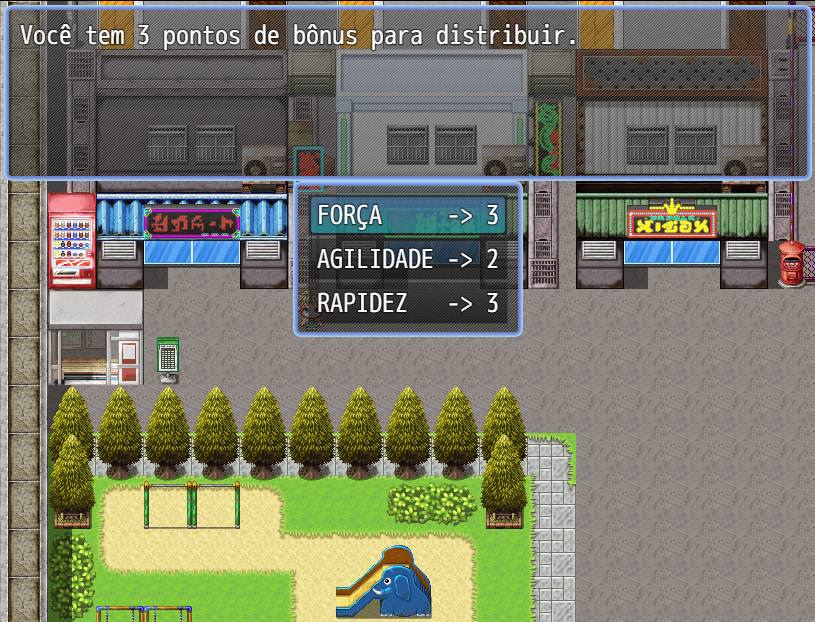
\includegraphics[scale=0.55]{Textuais/Pictures/Distribui-bonus.png}
	\fonte{Elaborado pelo autor (2023).}\label{fig:distribui-bonus}
\end{figure}

\newpage

Após a distribuição dos pontos de bônus, o jogador é inserido na narrativa, onde necessita tomar decisões cruciais. A primeira decisão é a escolha de um relógio: um modelo funcional e econômico por R\$ 30,00 ou o relógio do Major Trovão, mais caro R\$ 45,00 e popular entre os colegas. Essa escolha, conforme ilustrado na figura~\ref{fig:escolha-relogio}, influencia o desenrolar da história, pois a aquisição do relógio mais caro limita os recursos financeiros para a compra de outros itens, como a lanterna necessária para a exploração do porão.

\begin{figure}[!htbp]
	\centering
	\caption{Escolha do relógio.}
	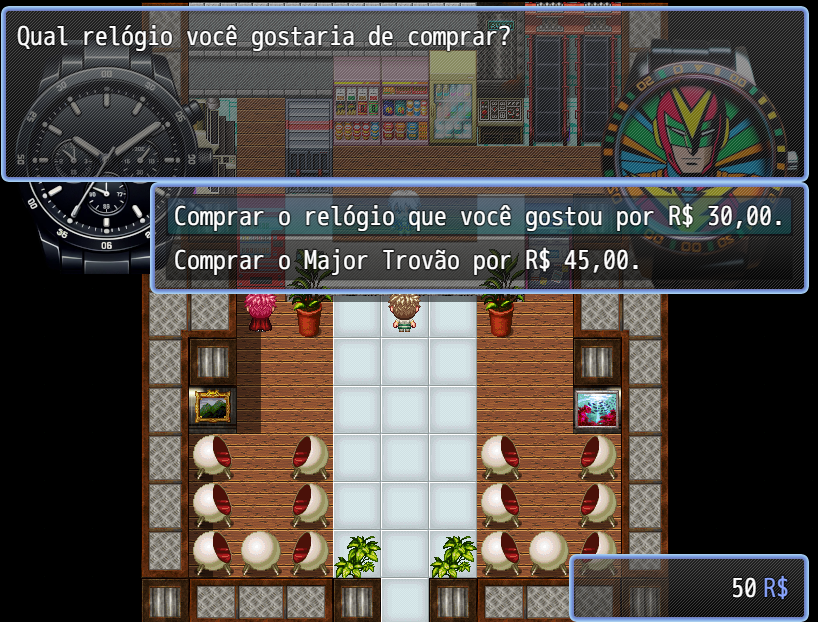
\includegraphics[scale=0.5]{Textuais/Pictures/escolha-relogio.png}
	\fonte{Elaborado pelo autor (2023).}\label{fig:escolha-relogio}
\end{figure}

Posteriormente, o jogador se dirige à lanchonete para um encontro com amigos, ocasião em que gasta R\$ 5,00. Esta etapa é retratada na figura~\ref{fig:lanchonete-pos-relogio}, e dependendo da escolha do relógio, o jogador pode ter recursos limitados, conforme demonstrado na figura~\ref{fig:lanchonete-pos-relogio-mt}.

\begin{figure}[!htbp]
	\centering
	\caption{Lanche pós-escolha do relógio econômico.}
	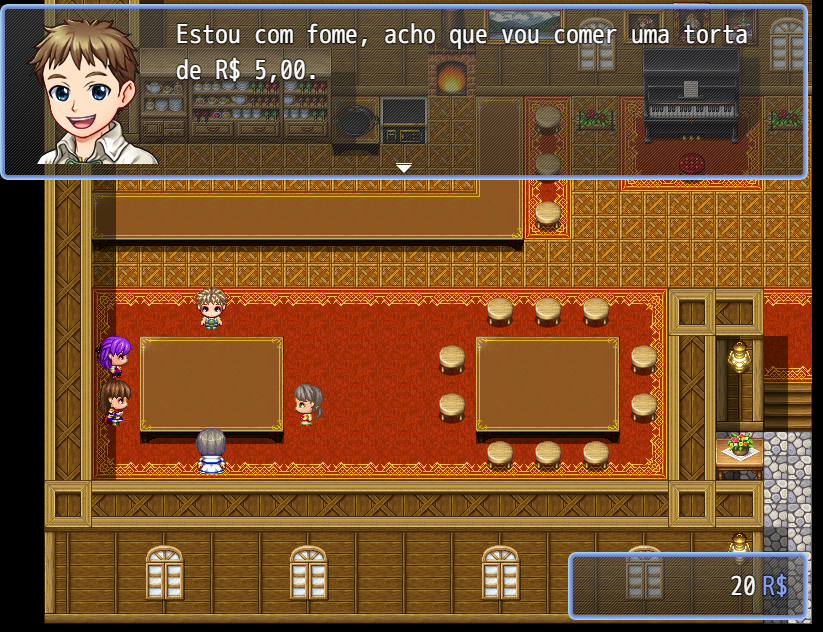
\includegraphics[scale=0.5]{Textuais/Pictures/lanchonete-pos-relogio.png}
	\fonte{Elaborado pelo autor (2023).}\label{fig:lanchonete-pos-relogio}
\end{figure}

\begin{figure}[!htbp]
	\centering
	\caption{Lanche após a compra do relógio Major Trovão.}
	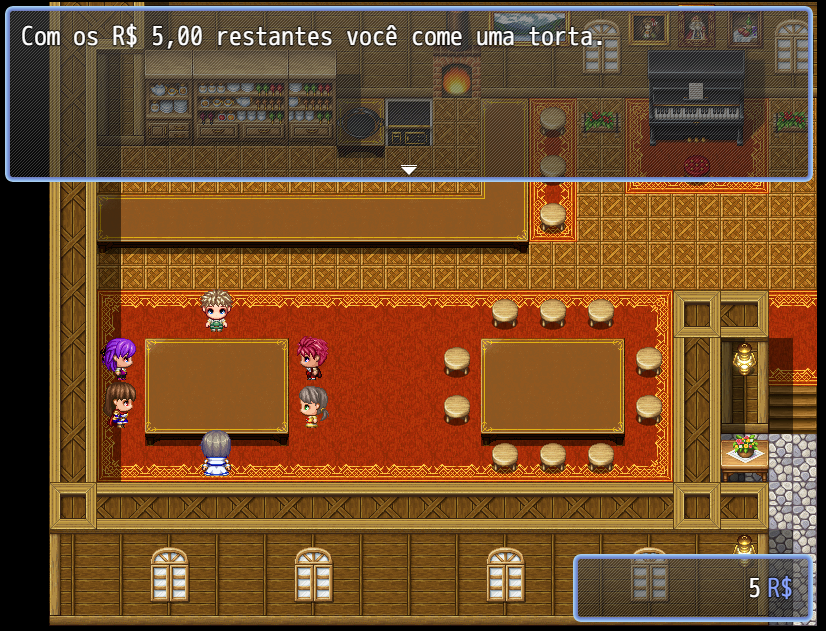
\includegraphics[scale=0.5]{Textuais/Pictures/lanchonete-pos-relogio-mt.png}
	\fonte{Elaborado pelo autor (2023).}\label{fig:lanchonete-pos-relogio-mt}
\end{figure}

\newpage

A próxima fase do jogo envolve a compra de uma lanterna por R\$ 10,00, essencial para investigar o porão da papelaria. A capacidade do jogador de adquirir a lanterna depende das escolhas financeiras anteriores, como representado nas figuras~\ref{fig:compra-lanterna} e~\ref{fig:nao-compra-lanterna}.

\begin{figure}[!htbp]
	\centering
	\caption{Aquisição da lanterna.}
	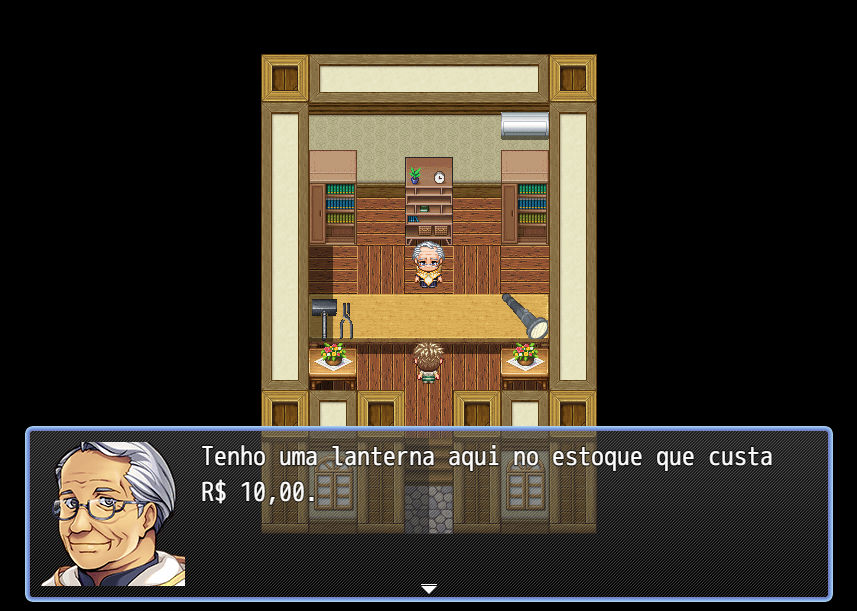
\includegraphics[scale=0.5]{Textuais/Pictures/compra-lanterna.png}
	\fonte{Elaborado pelo autor (2023).}\label{fig:compra-lanterna}
\end{figure}

\begin{figure}[!htbp]
	\centering
	\caption{Incapacidade de comprar a lanterna.}
	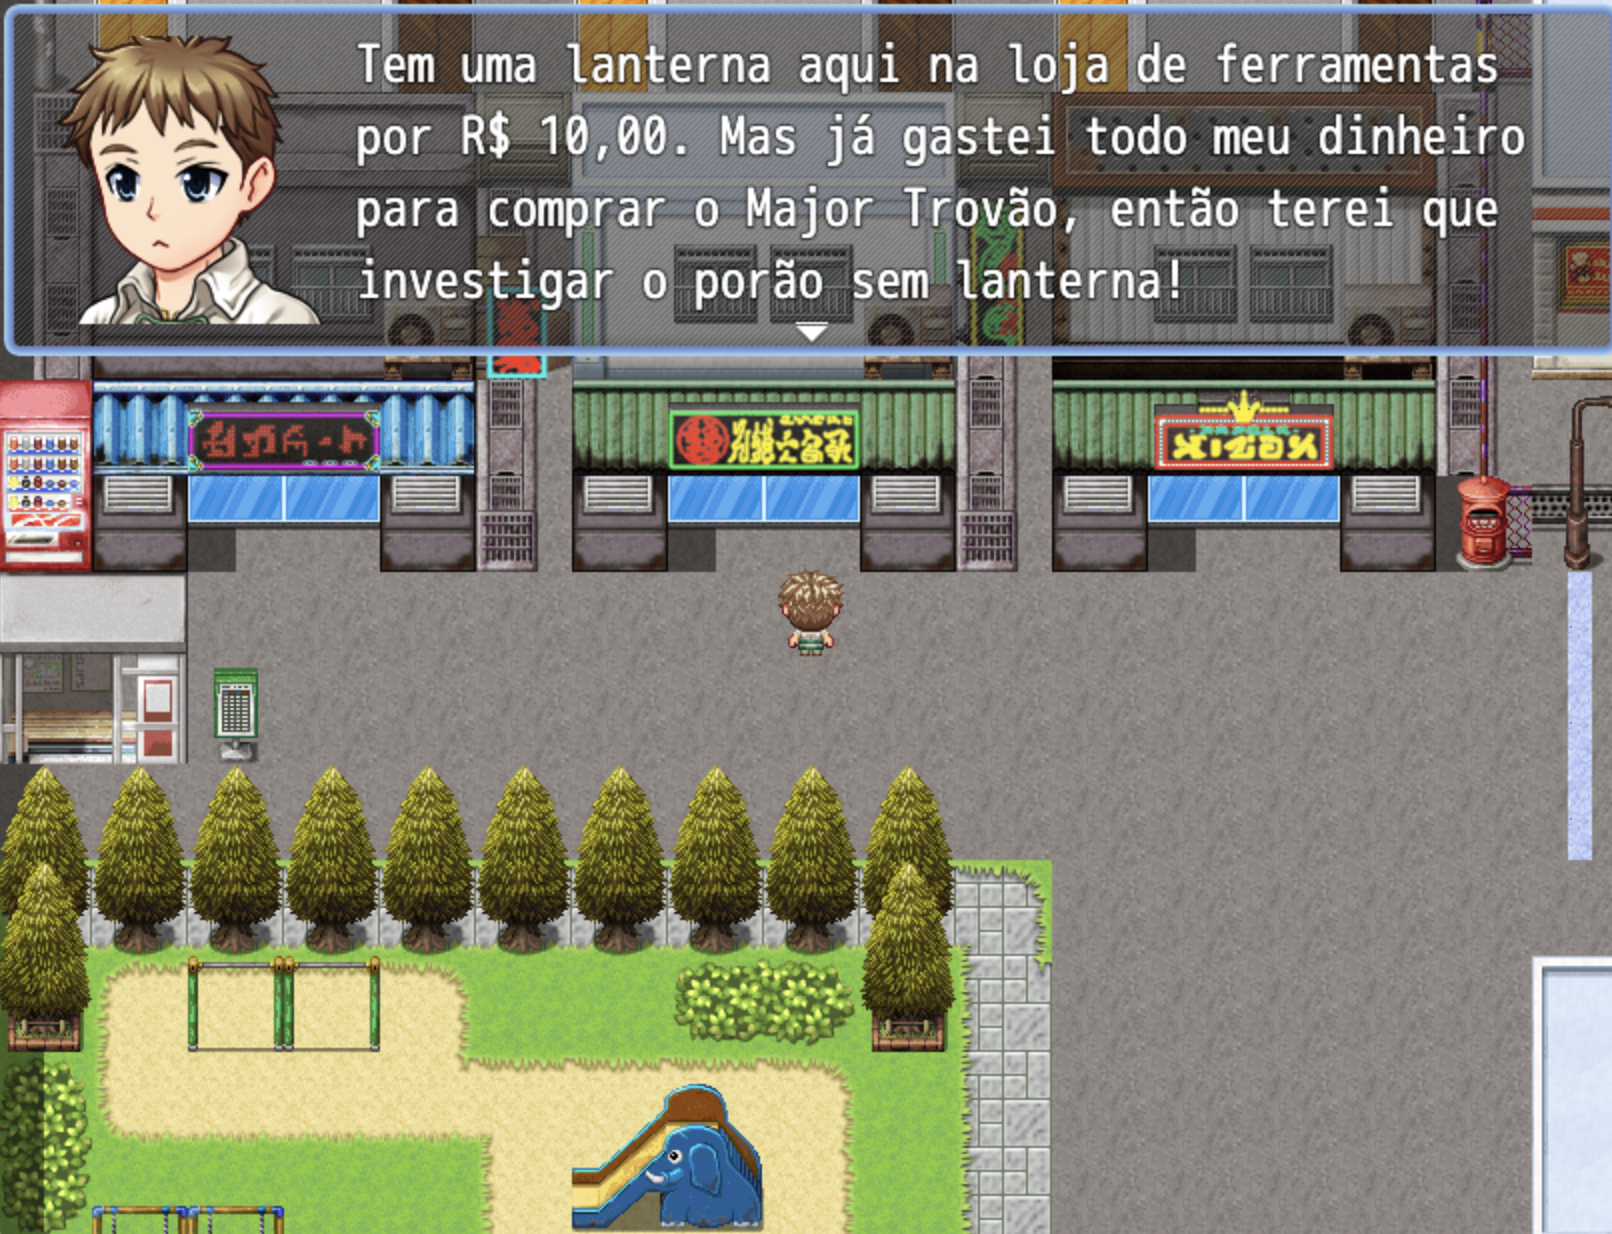
\includegraphics[scale=0.4]{Textuais/Pictures/nao-compra-lanterna.png}
	\fonte{Elaborado pelo autor (2023).}\label{fig:nao-compra-lanterna}
\end{figure}

Após a aquisição (ou não) da lanterna, o personagem principal chega à papelaria e se depara com um barulho na cozinha. Nesse momento, é apresentada uma escolha crítica ao jogador, como ilustra a figura~\ref{fig:chega-cozinha-papelaria}: investigar a cozinha ou prosseguir diretamente para o porão.

\begin{figure}[!htbp]
	\centering
	\caption{Decisão entre investigar a cozinha ou ir direto ao porão.}
	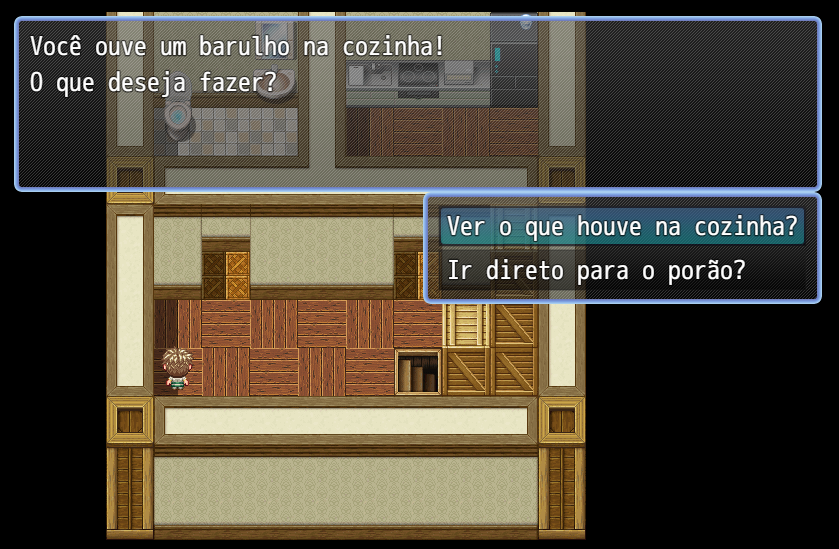
\includegraphics[scale=0.45]{Textuais/Pictures/chega-cozinha-papelaria.png}
	\fonte{Elaborado pelo autor (2023).}\label{fig:chega-cozinha-papelaria}
\end{figure}

Na cozinha, o jogador encontra Josimar e, após sua saída, descobre um problema na geladeira que gera desperdício de energia. Esta descoberta é representada na figura~\ref{fig:desperdicio-geladeira}.

\begin{figure}[!htbp]
	\centering
	\caption{Descoberta do desperdício de energia pela geladeira.}
	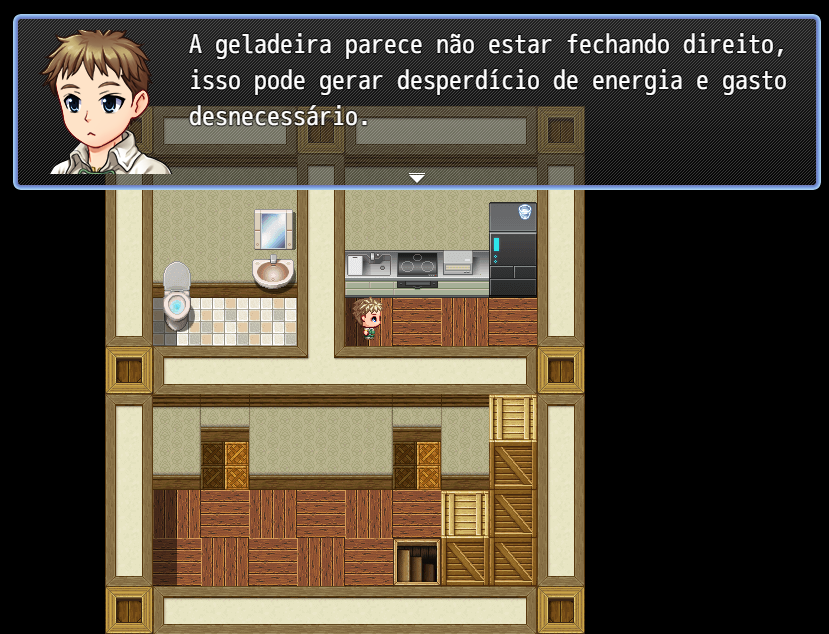
\includegraphics[scale=0.45]{Textuais/Pictures/desperdicio-geladeira.png}
	\fonte{Elaborado pelo autor (2023).}\label{fig:desperdicio-geladeira}
\end{figure}

A exploração do porão pode ocorrer com ou sem a lanterna, conforme as figuras~\ref{fig:explorando-porao-com-lanterna} e~\ref{fig:explorando-porao-sem-lanterna} demonstram. A falta de lanterna e uma baixa pontuação em agilidade podem levar a um ataque de ratazana, culminando em um final prematuro do jogo, como mostrado na figura~\ref{fig:game-over}.

\begin{figure}[!htbp]
	\centering
	\caption{Exploração do porão com a lanterna.}
	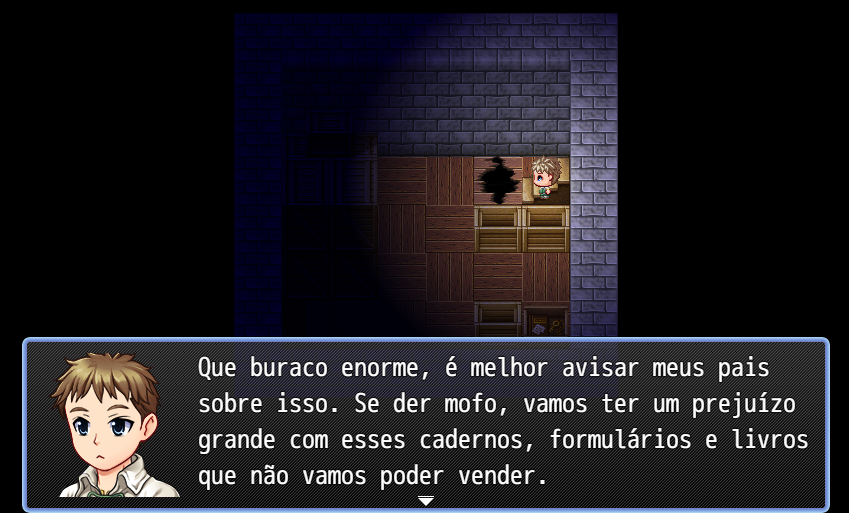
\includegraphics[scale=0.55]{Textuais/Pictures/explorando-porao-com-lanterna.png}
	\fonte{Elaborado pelo autor (2023).}\label{fig:explorando-porao-com-lanterna}
\end{figure}

\begin{figure}[!htbp]
	\centering
	\caption{Exploração do porão sem a lanterna.}
	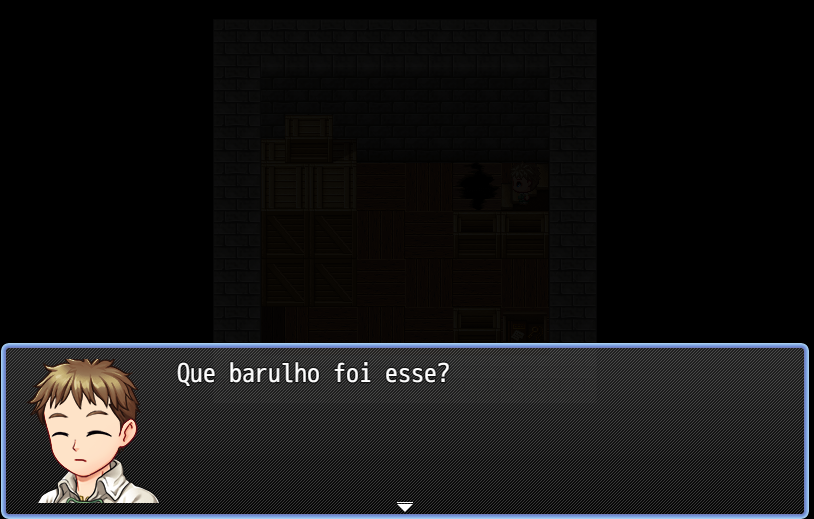
\includegraphics[scale=0.55]{Textuais/Pictures/explorando-porao-sem-lanterna.png}
	\fonte{Elaborado pelo autor (2023).}\label{fig:explorando-porao-sem-lanterna}
\end{figure}

\begin{figure}[!htbp]
	\centering
	\caption{Consequências de uma baixa pontuação em agilidade.}
	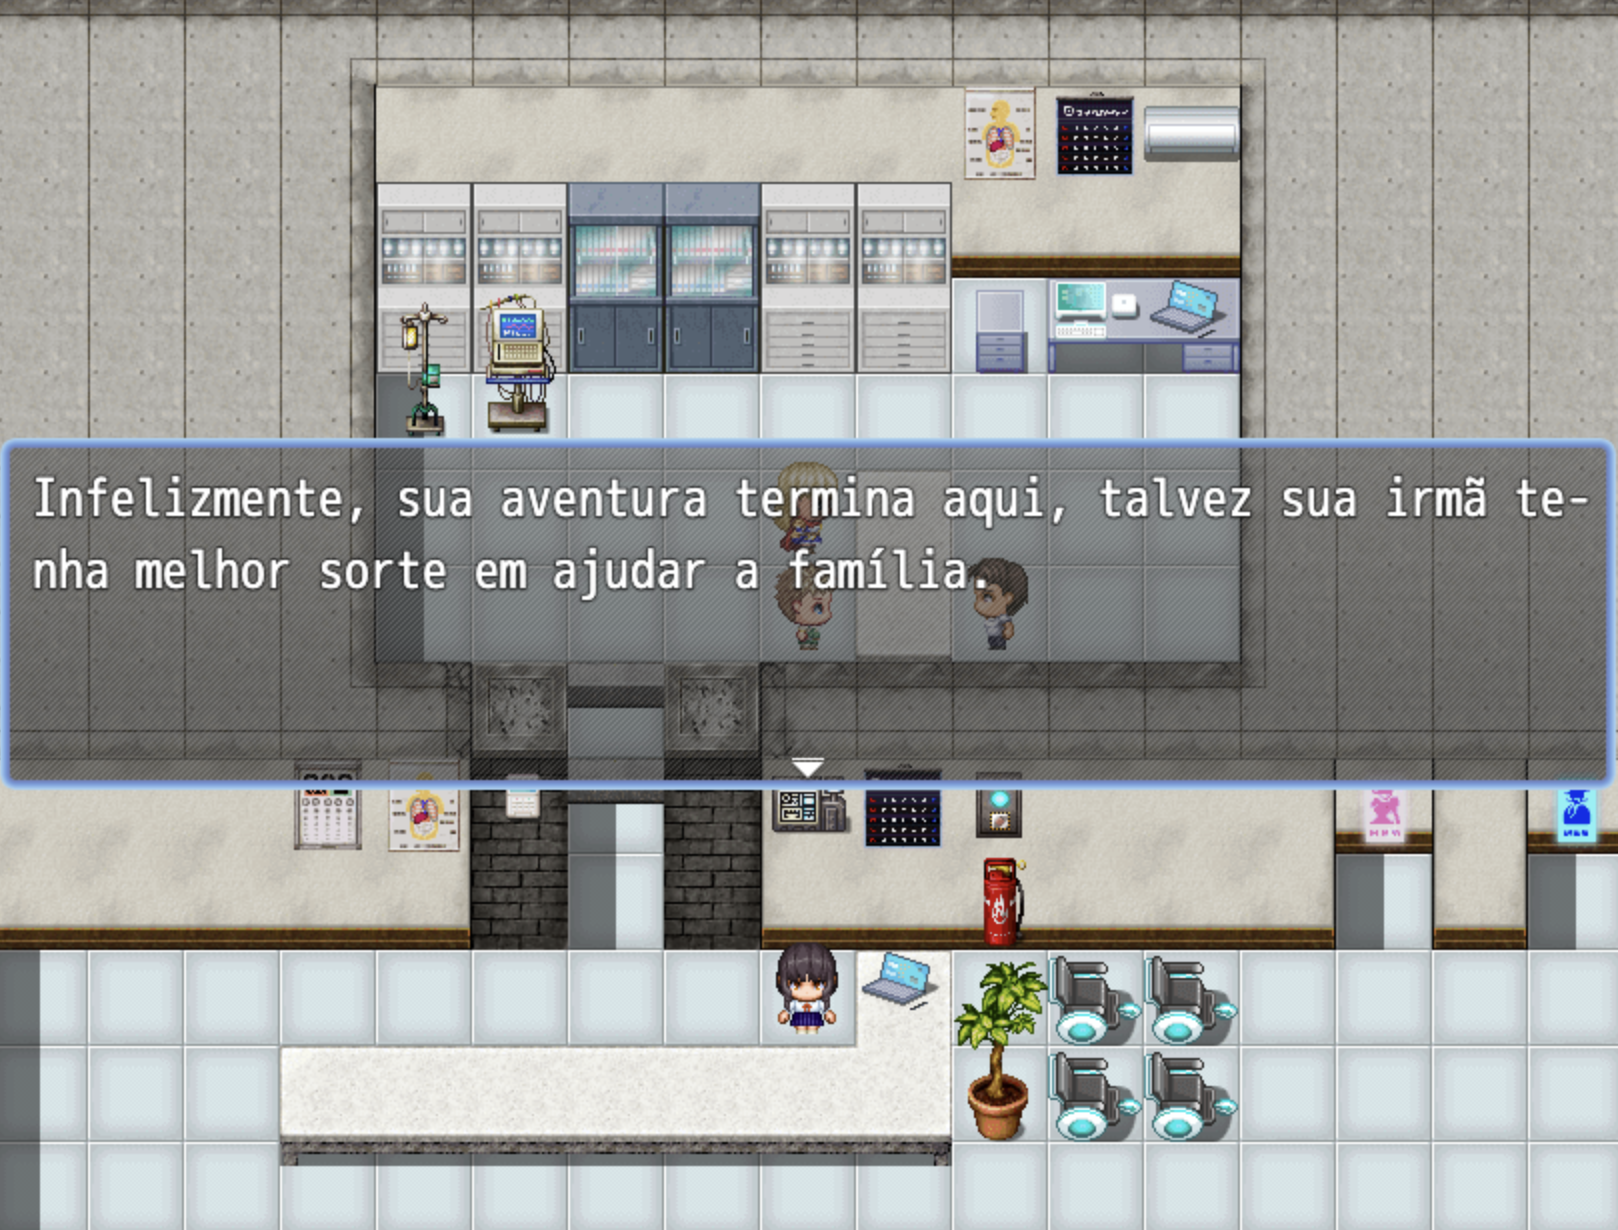
\includegraphics[scale=0.4]{Textuais/Pictures/game-over.png}
	\fonte{Elaborado pelo autor (2023).}\label{fig:game-over}
\end{figure}

\newpage
\newpage

Se o jogador realizar escolhas adequadas ao longo do jogo, alcança um desfecho positivo. A família descobre a origem dos problemas financeiros e encontra moedas esquecidas, solucionando o mistério. Este desfecho vitorioso é ilustrado na figura~\ref{fig:vitoria}.

\begin{figure}[!htbp]
	\centering
	\caption{Conclusão bem-sucedida do jogo.}
	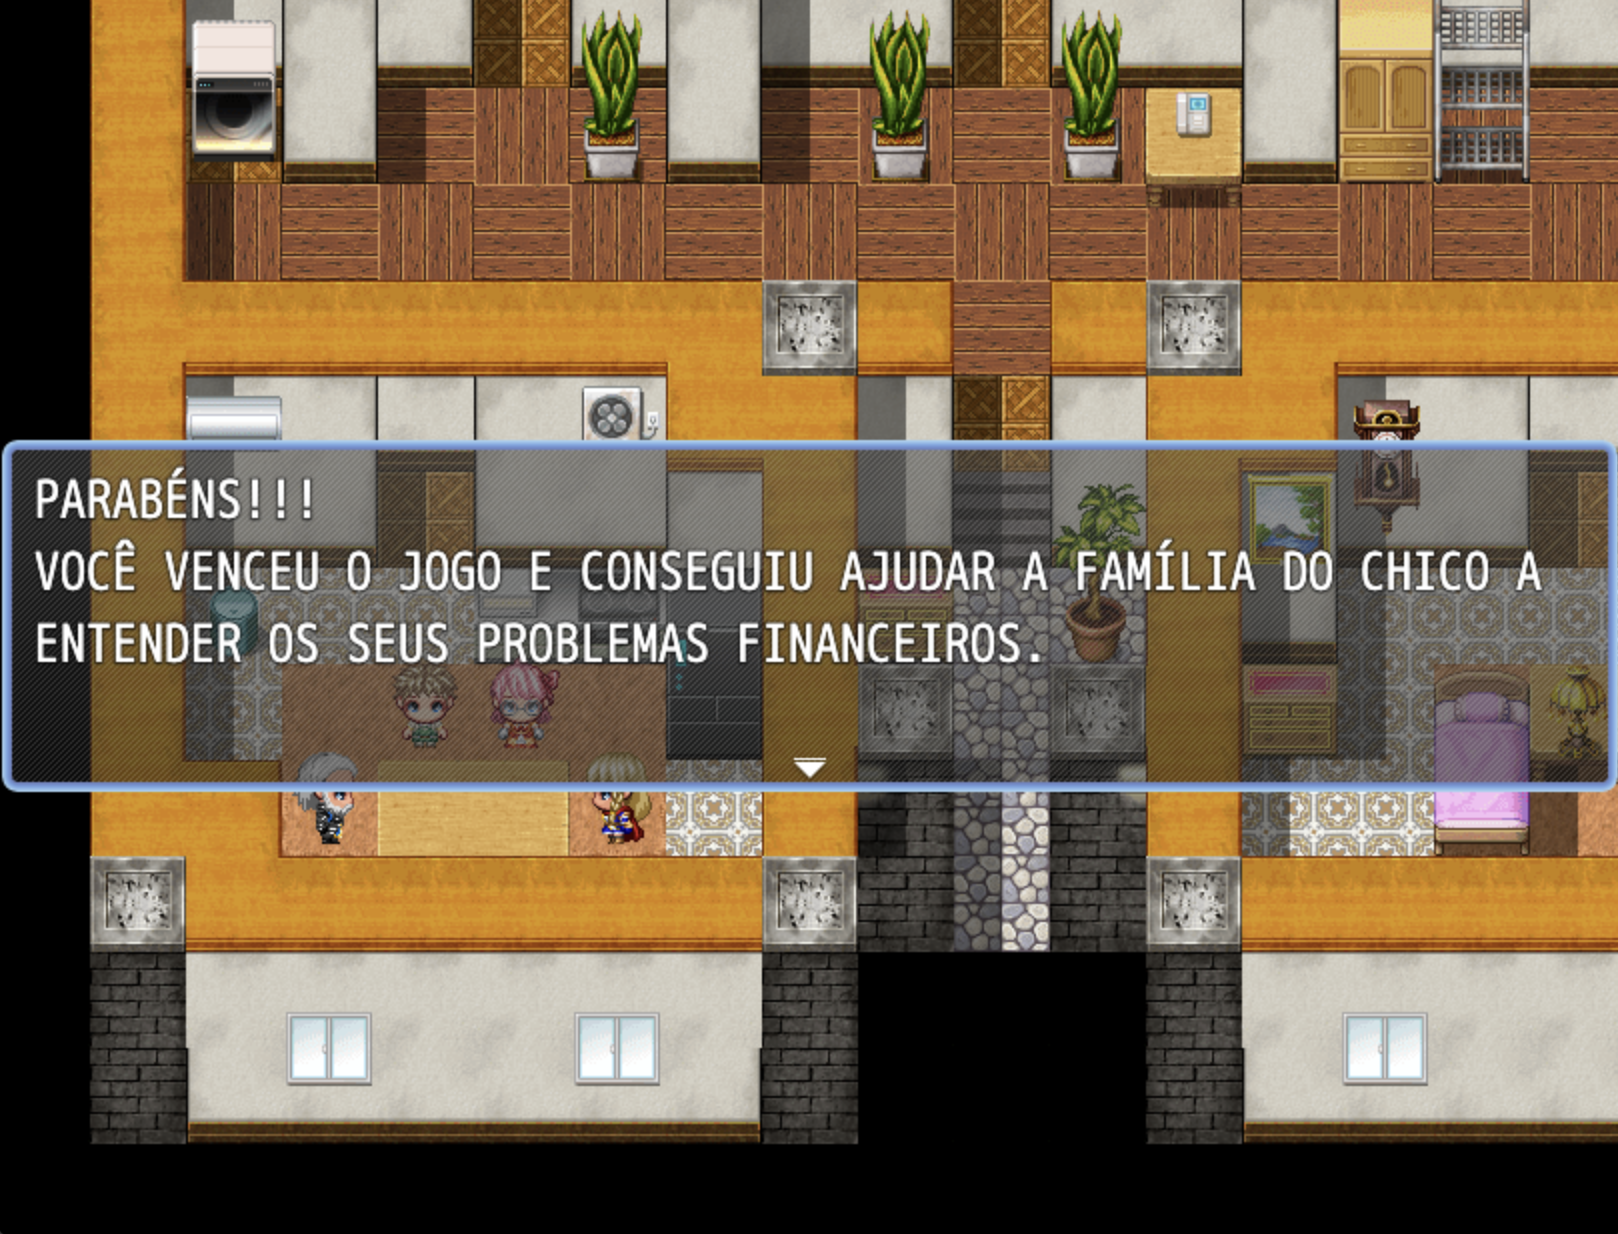
\includegraphics[scale=0.4]{Textuais/Pictures/vitoria.png}
	\fonte{Elaborado pelo autor (2023).}\label{fig:vitoria}
\end{figure}

\section{Análise Crítica do Jogo Mistério Financeiro: A Jornada de Chico}

\subsection*{Público-Alvo}
O jogo "Mistério Financeiro" é direcionado para crianças do 5º ano do Ensino Fundamental, demandando abordagens educativas lúdicas e interativas. Este foco no público infantil distingue-o de jogos como \textit{Debt Maze}~\ref{subsec:debt-maze} e \textit{Finance Game}~\ref{subsec:finance-game}, mais apropriados para adultos ou adolescentes.

\subsection*{Metodologia de Ensino}
Ao contrário do \textit{PlanCash}~\ref{subsec:plancash}, que utiliza uma estrutura de jogo de tabuleiro, e do \textit{InvestPlay}~\ref{subsec:investplay}, baseado em perguntas e respostas, "Mistério Financeiro" emprega uma narrativa interativa RPG. Esta abordagem é particularmente eficaz para engajar crianças mais novas.

\subsection*{Abordagem Pedagógica}
O jogo promove aprendizagem por meio da exploração e tomada de decisões, similar ao \textit{Debt Maze}~\ref{subsec:debt-maze}, mas de uma forma mais acessível e relevante para o público infantil. As situações financeiras são integradas naturalmente na narrativa, facilitando a compreensão e retenção de conhecimento.

\subsection*{Imersão Narrativa}
A rica narrativa de Chico e sua família em "Mistério Financeiro" oferece uma experiência imersiva, em contraste com o \textit{PlanCash}~\ref{subsec:plancash}, cujo formato de jogo de tabuleiro pode limitar o envolvimento narrativo.

\subsection*{Contextualização Cultural e Linguística}
O "Mistério Financeiro" destaca-se pela sua forte contextualização no cenário brasileiro e uso do português como idioma principal, diferenciando-se de jogos como o \textit{Debt Maze}~\ref{subsec:debt-maze}, que apresentam barreiras linguísticas para o público brasileiro.

\subsection*{Aderência à ENEF}
Este jogo está alinhado com os princípios da Estratégia Nacional de Educação Financeira (ENEF), ao contrário de outros jogos analisados. Esta conformidade assegura que o conteúdo e as lições financeiras estejam em harmonia com os objetivos educacionais nacionais.

\subsection*{Pontos Fracos}
O "Mistério Financeiro", apesar de suas vantagens, ainda carece de avaliação empírica com alunos, limitando a validação de sua eficácia educacional. Além disso, a narrativa específica pode restringir a re-jogabilidade e a variedade dos cenários financeiros explorados.

A análise comparativa revela que o "Mistério Financeiro" oferece uma abordagem inovadora e adequada para o seu público-alvo, distinguindo-se significativamente dos outros jogos analisados em termos de metodologia, abordagem pedagógica, imersão narrativa, contextualização cultural e aderência à ENEF. Cada jogo tem suas forças, mas o "Mistério Financeiro" ressalta-se pela sua integração única de educação financeira com uma narrativa envolvente, ajustada ao contexto cultural brasileiro.
